% This file demonstrates how to use the IEEEConf LaTeX2e macro package,
% to prepare a manuscript for proceedings on CD of the conference
% FedCSIS %VERA: hier arbeiten Deadline 2.Maiwoche
%
\documentclass[conference]{IEEEtran} % ,onecolumn
%\documentclass[a4paper]{IEEEconf}

% This package serves to balance the column lengths on the last page of the document.
% please, insert \balance command in the left column of the last page
\usepackage{balance}
\usepackage[utf8]{inputenc}
\usepackage{tabularx}

%% to enable \thank command
\IEEEoverridecommandlockouts 
%% The usage of the following packages is recommended
%% to insert graphics
\usepackage[dvips]{graphicx}
% to typeset algorithms
\usepackage{algorithmic}
\usepackage{algorithm}
% to typeset code fragments
\usepackage{listings}
% to make an accent \k be available
%\usepackage[OT4,T1]{fontenc}
% provides various features to facilitate writing math formulas and to improve the typographical quality of their output.
\usepackage[cmex10]{amsmath}
\interdisplaylinepenalty=2500
% por urls typesetting and breaking
\usepackage{url}
% for vertical merging table cells
\usepackage{multirow}
\usepackage{pgfplots} 
% define environments for remarks and examples
%\newtheorem{remark}{Remark}[section]
\newtheorem{remark}{Remark}[section]
\newtheorem{example}[remark]{Example}
\usepackage{amssymb}
\usepackage{amsthm}
\newtheorem{definition}{Definition}
\newtheorem{dfn}{Definition}
\newtheorem{thm}[dfn]{Theorem}
\newtheorem{corollary}[dfn]{Corollary}
\newtheorem{exl}[dfn]{Example}
\newtheorem{lem}[dfn]{Lemma}
%
%
\title{Towards the analysis of errors in centrality measures in perpetuated networks}
%
%
\author{
\IEEEauthorblockN{Meetkumar Pravinbhai Mangroliya\IEEEauthorrefmark{1}%\IEEEauthorrefmark{3}
, Jens D\"orpinghaus\IEEEauthorrefmark{1}\IEEEauthorrefmark{2}, Robert Rockenfeller\IEEEauthorrefmark{1}}%, Vera Weil\IEEEauthorrefmark{3}}
\IEEEauthorblockA{%
\IEEEauthorrefmark{1}  University of Koblenz, Germany\\ Email: meetmangroliya987@uni-koblenz.de, \url{https://orcid.org/0009-0003-3727-9527}}
\IEEEauthorrefmark{2} Federal Institute for Vocational Education and Training (BIBB), Bonn, Germany\\ Email: jens.doerpinghaus@bibb.de, \url{https://orcid.org/0000-0003-0245-7752}
}

%\IEEEauthorblockA{%
%\IEEEauthorrefmark{3} University of Pretoria, Faculty of Theology and Religion, Hatfield, Pretoria, South Africa}
%}
% conference papers do not typically use \thanks and this command
% is locked out in conference mode. If really needed, such as for
% the acknowledgment of grants, issue a \IEEEoverridecommandlockouts
% after \documentclass

% for over three affiliations, or if they all won't fit within the width
% of the page, use this alternative format:
% 
%\author{\IEEEauthorblockN{Michael Shell\IEEEauthorrefmark{1},
%Homer Simpson\IEEEauthorrefmark{2},
%James Kirk\IEEEauthorrefmark{3}, 
%Montgomery Scott\IEEEauthorrefmark{3} and
%Eldon Tyrell\IEEEauthorrefmark{4}}
%\IEEEauthorblockA{\IEEEauthorrefmark{1}School of Electrical and Computer Engineering\\
%Georgia Institute of Technology,
%Atlanta, Georgia 30332--0250\\ Email: see http://www.michaelshell.org/contact.html}
%\IEEEauthorblockA{\IEEEauthorrefmark{2}Twentieth Century Fox, Springfield, USA\\
%Email: homer@thesimpsons.com}
%\IEEEauthorblockA{\IEEEauthorrefmark{3}Starfleet Academy, San Francisco, California 96678-2391\\
%Telephone: (800) 555--1212, Fax: (888) 555--1212}
%\IEEEauthorblockA{\IEEEauthorrefmark{4}Tyrell Inc., 123 Replicant Street, Los Angeles, California 90210--4321}}


%\newtheorem{dfn}{Definition}[section]
%\newtheorem{thm}[dfn]{Theorem}
%\newtheorem{exl}[dfn]{Example}
%\newtheorem{lem}[dfn]{Lemma}
\newcommand{\IS}{\mathbb{S}}
\newcommand{\IN}{\mathbb{N}}


\begin{document}
\maketitle              % typeset the title of the contribution

\begin{abstract}
Centrality measures are essential tools for analyzing the structure and dynamics of graphs, such as knowledge or social networks. They reveal the significance and influence of individual nodes. However, their accuracy can be influenced by data quality, algorithms, and network properties. This study investigates errors in centrality measures within perpetuated networks. It focuses on network resilience and how these results may be used to develop efficient algorithms for centrality measures. It also investigates how perturbation strategies impact network resilience and predict connectivity in the perturbed network. By employing centrality measures (degree, betweenness, closeness, eigenvector), we identify critical nodes that significantly affect network connectivity and information flow. Additionally, statistical tests (Kolmogorov-Smirnov, Cramér-von Mises) assess network robustness and pinpoint critical transition points. This study, by outlining methods for error identification, quantification, and mitigation, offers valuable insights for enhancing network resilience across various domains, including infrastructure design and social network analysis.
\end{abstract}

\begin{IEEEkeywords}
Centrality Measures, Complex Networks, Social Network Analysis, Optimization on graphs
\end{IEEEkeywords}

\section{Introduction}

In the contemporary era, networks are pervasively present. These networks may be tangible systems, such as power grids or transportation networks, or they may be abstract entities, such as networks of acquaintances or collaborations. As individuals, we are all interconnected within a network of social relationships \cite{boccaletti2006complex,dorpinghaus2022social}.

In network analysis, centrality measures provide crucial quantitative tools for assessing the importance of individual nodes within a network \cite{borgatti2005centrality, newman2010networks,dorpinghaus2022context,dorpinghaus2023towards} and are also used for AI, e.g., link prediction methods \cite{dorpinghaus2022novel,dahhani2023graph}. Among these measures, degree centrality is particularly significant. Degree centrality quantifies the importance of a node by counting the number of direct connections it has to other nodes in the network, thus reflecting its immediate influence within the network structure \cite{freeman1978centrality}. To comprehend the resilience of networks to disruptions, perturbation strategies play a pivotal role \cite{albert2000error, newman2010networks}. These strategies entail the selective or random removal of nodes or edges from a network, with the objective of studying the impact of such removals on the network's structure and properties. In particular, we focus on four removal strategies: high-degree node removal, low-degree node removal, random node removal, and random edge removal. By evaluating the change in degree centrality before and after employing these strategies, we gain insights into the relative importance of different nodes and edges in maintaining the network's overall structure and function \cite{newman2010networks, borgatti2005centrality}. This is our first research question. 

Furthermore, as a second research question, we aim to identify the critical points at which the removal of a node or edge causes the network to be fragmented and undergo significant structural changes. This information is crucial for domains that rely on network connectivity and stability, such as telecommunications and social science, as it provides insights into how these networks might be susceptible to disruption and how their resilience can be enhanced \cite{albert2000error, newman2010networks}. By understanding these critical points, we can proactively develop strategies to improve the networks' resilience to potential failures and improve their overall robustness.

To evaluate these changes statistically, the Kolmogorov-Smirnov (K-S) and Cramér-von Mises (CvM) tests are employed \cite{broido2019scale, arnold2011nonparametric}. These non-parametric statistical tests are used to compare the degree distribution - the distribution of node degrees, representing the number of connections each node has - of a network before and after removal and show the significant change in the structure. To our knowledge, only a few studies have employed the Kolmogorov-Smirnov (KS) test to assess the differences in the degree distributions of networks \cite{clauset2009power, broido2019scale}. However, no studies have employed the Cramér-von Mises (CvM) test for this purpose. This chapter serves as the foundation for our study, laying the groundwork for exploring types of complex networks and utilizing various tools to deepen our understanding.

Following the introduction, this study is structured into four sections. The second section presents a comprehensive review of relevant literature on centrality measures, perturbation strategies, and network resilience, establishing the theoretical and empirical foundation. The third section details the methodology, outlining data collection, analysis, and statistical evaluation procedures. The fourth section presents and analyzes the experimental results, detailing the effects of different removal strategies on network properties. Finally, the fifth section presents a discussion and outlook, interpreting the results, drawing conclusions, and proposing future research directions to advance the understanding of network dynamics and resilience.

\section{Related Work}

\subsection{Network Perturbation}

Networks are both resilient and fragile, meaning that they can withstand some perturbations but are also vulnerable to others. Node and edge removal is a technique that can be used to study how these networks respond to perturbations. Node and edge removal analysis has a rich history in network science. By systematically removing nodes or edges, we gain a deeper understanding of network robustness and efficiency. It is also worth noting that similar questions are addressed within the field of longitudinal network analysis, see \cite{dorpinghaus2023towards}. 

Modern research examines deeper into the intricate interplay between network structure, dynamics, and resilience under various removal scenarios. Additionally, advancements in machine learning and computational techniques have allowed for the development of predictive models to estimate the impacts of node and edge removal before they are executed, enhancing our ability to formulate proactive strategies for network optimization and management. We can use mathematical models, optimization algorithms, and simulations to study the removal of nodes and edges from a network and to predict the effects of these removal actions.

Researchers have proposed and explored diverse methods for removing nodes and edges, encompassing strategies like random removal \cite{albert2000error, albert2002statistical}, as well as centrality-based removals such as degree centrality and betweenness centrality \cite{wandelt2018comparative, inbook}. A prevalent attack strategy involves pinpointing critical nodes based on metrics like degree or other centrality measures and systematically removing them in descending order of importance until the network either disconnects or loses essential properties \cite{holme2002attack}. Albert's investigation into the fragmentation of random and scale-free networks employed two distinct node removal strategies: targeted removal (attacks) and random removal (errors) \cite{albert2000error}. In the research of Smith et al. \cite{smith2015edge}, the authors systematically eliminated genes from a biological network to examine the consequences on both network connectivity and behavior. Additionally, in the study of Bellingeri et al. \cite{bellingeri2020comparative}, the authors performed a comparative analysis to evaluate the effects of diverse link removal strategies on various real-world complex networks. Additionally, numerous studies have examined the impact of removal strategies on complex networks across various scientific domains \cite{latora2001efficient, yang2017small, caldu2018structural, gallos2005stability, zanin2013modelling,dorpinghaus2022centrality}. These methodologies provide a comprehensive understanding of how the removal of nodes and edges influences the overall structure and functionality of networks.

\subsection{Impact on Network Connectivity and Structure}

Network connectivity is essential for any network. It allows information, influence, resources, and even diseases to flow between the nodes of the network. In other words, network connectivity is what makes networks useful and powerful. Without connectivity, networks would be nothing more than a collection of isolated nodes \cite{newman2010networks}. Studying how removing nodes and edges from a network affects its ability to connect its nodes is not just a theoretical exercise rather, it can help us to understand how complex systems work and how to make them more resilient. We can identify the vulnerabilities of complex systems by identifying the nodes and edges that are essential for the network's functioning. We can also identify the types of failures that are most likely to occur in a network. 

Moreover, structural changes within networks, whether through the addition or removal of nodes and edges or alterations in degree distribution, can profoundly impact their overall connectivity and efficiency \cite{albert2000error, schneider2011mitigation}. The effects of node and edge removal on network connectivity have been a subject of extensive research in the field of network science, various studies have explored the effects of perturbation strategies on network resilience and structure. Albert et al. \cite{albert2000error} investigated the contrasting vulnerabilities of scale-free and random networks to node perturbation. Holme et al. \cite{holme2002attack} examined the susceptibility of complex networks to targeted perturbation, while Bellingeri et al. \cite{Bellingeri_2014} studied attack strategies in real-world networks. Wandelt et al. \cite{wandelt2018comparative} compared network dismantling strategies, finding node removal often outperforms edge removal, with hybrid approaches effective in specific cases. Callaway et al. \cite{callaway2000network} analyzed network resilience to failures and attacks, and Chen and Li \cite{chen2019community} explored community detection using constrained edge-deleting strategies, demonstrating potential for increased robustness. 

After reviewing the work of these researchers in this field, we aim to explore how different node perturbation strategies, including targeted and random perturbation, influence network connectivity.

However, studying the impact of node and removal on different structures and connectivity is not without challenges. The interplay between local and global network structure presents complexities in predicting network behavior \cite{holme2002attack}. Furthermore, quantifying the impact of removal strategies on network robustness requires sophisticated algorithms and computational resources \cite{schneider2011mitigation}. Moreover, the ethical implications of removal actions in real-world networks, such as social networks, introduce ethical considerations \cite{baltar2012unintended}. Our research aims to navigate these challenges and contribute to a more comprehensive understanding of network connectivity and structural changes due to node and edge removal.

\subsection{Statistical Tests in Network Analysis}

In statistical hypothesis testing, the Cramér-von Mises (CvM) test and the Kolmogorov-Smirnov (K-S) test are two most popular non-parametric tests to evaluate the goodness-of-fit between two probability distributions \cite{arnold2011nonparametric}.

\subsubsection{Kolmogorov-Smirnov (K-S) test}

The Kolmogorov-Smirnov (K-S) test is a statistical tool employed to evaluate whether two cumulative distribution functions (CDF) differ significantly \cite{broido2019scale, arnold2011nonparametric}. It quantifies the maximum vertical difference between the CDF of the dataset of original degree distribution and the CDF of reduced degree distribution of the network after removal of nodes or edges \cite{broido2019scale, ksdegree2014,faloutsos1999structure}.

Let $F_{1,n}$ be the cumulative distribution function of original network with a number of nodes $n$ and $F_{2,m}$ be the cumulative distribution function of the network after node or edge removal with a remaining number of nodes $m$, then the K-S statistic, denoted as $D_{n,m}$, quantifies the maximum absolute difference between these functions, given by \cite{arnold2011nonparametric}:

\begin{equation}
D_{n,m} = \sup_x |F_{1,n}(x) - F_{2,m}(x)|
\end{equation}

In practice, the null hypothesis is rejected at a specified significance level $\alpha$ if $D_{n,m}$ exceeds a critical value or in other words, if the condition in following equation \ref{eq:2.11} satisfies \cite{arnold2011nonparametric}.

\begin{equation}\label{eq:2.11}
    D_{n,m} > c(\alpha) \cdot \sqrt \frac{n \cdot m}{n + m}
\end{equation}

The value of $c(\alpha)$ at specified significance level is tabulated in \cite{table_crit_values_ks}. The highest vertical difference between the two distribution functions is quantified by the K-S statistic ($D_{n,m}$). A significant difference between the original and modified degree distributions is shown by a high K-S statistic and a low related p-value in the context of network analysis, suggesting that the removal approach has significantly affected the network's structure.

The KS test is particularly suitable for comparing network degree distributions as it doesn't necessitate any assumptions regarding the underlying distribution of the data \cite{clauset2009power, ksdegree2014}. The K-S test is exact and straightforward to interpret, delivering dependable outcomes even when dealing with small sample sizes \cite{EngineeringStatisticsHandbook}. This precision proves advantageous, especially in situations with constrained data \cite{kossinets2006empirical, newman2010networks}.

In the analysis of an evolving social network, Kossinets and Watts employed the Kolmogorov-Smirnov (K-S) test to compare the degree distributions of the network at different time points to identify and quantify the changes in the network's structure over time \cite{kossinets2006empirical}. Their work highlighted the potential of the K-S test for analyzing the evolution of complex networks over time. 

\subsubsection{Cramér-von Mises Test}

The Cramér-von Mises (CvM) test is another statistical method used for comparing the empirical cumulative distribution function (ECDF) of the sample to the cumulative distribution function (CDF) of a hypothesized distribution. The Cramér-von Mises $W^2$ criterion is named after Harald Cramér \cite{cramer1928composition} and Richard Edler von Mises \cite{vonmises1928wahrscheinlichkeit}. According to Anderson \cite{anderson1962distribution}, the Cramér-von Mises $W^2$ criterion for testing that a sample, $x_1, x_2, \ldots$, has been drawn from a specified continuous distribution $F(x)$ is:
\[
W^2 = \int_{-\infty}^{\infty} [F_N(X) - F(x)]^2 \, dF(x),
\]
where $F_N(X)$ is the empirical distribution function of the sample. For a second sample, $y_1, y_2, \ldots, y_M$, a test of the hypothesis that the two samples come from the same (unspecified) continuous distribution can be based on the analogue of $W^2$, namely
\[
T = \frac{NM}{N + M} \int_{-\infty}^{\infty} [F_N(x) - G_M(x)]^2 \, dH_{N+M}(x),
\]
where $G_M(x)$ is the empirical distribution function of the second sample and $H_{N+M}(x)$ is the empirical distribution function of the two samples together.

If the computed value of $T$ gets higher than the tabulated critical values from \cite{anderson1962distribution} then the null hypothesis that the two samples come from the same distribution can be rejected in the favour of alternative hypothesis. The CvM statistic ($T$) provides a measure of dissimilarity between the two samples.

It is general understanding that the Cramér-von Mises (CvM) test is considered a good choice for comparing distributions with heavy tails compared to the Kolmogorov-Smirnov (K-S) test due to its sensitivity to deviations in the tails of the distribution where crucial information about the network's structure is often contained \cite{stephens1974edf}. There is only few studies that have employed the K-S test as the statistical tool to assess the differences in the degree distribution of the network and none to our knowledge that have employed CvM test.

\section{Method}
In our analysis, we employ a systematic methodology to generate three types of complex networks and investigate the influence of node and edge removal strategies on centrality measures within these networks. We focus on the fundamental centrality measure—degree centrality, due to its distinct and complementary perspectives on node importance within networks. Degree centrality is computed using the NetworkX library in Python, which offers efficient implementations of various centrality algorithms \cite{hagberg2008exploring}. This measure provides valuable insights into the structural significance of nodes within complex networks.

\subsection{Generation of Complex Networks}

A random network was generated using the Erdős-Rényi (ER) graph generator from the NetworkX library \cite{hagberg2008exploring}. The network parameters were set to include 100 nodes (n) and an edge probability of 0.2 (p) \cite{erdos1959random, gilbert1959random}. This edge probability influences the network's density, with higher values resulting in denser networks and lower values yielding sparser ones. Additionally, Python's random state function was used to establish a consistent random seed (seed = 1) for reproducible network generation.

The Barabási-Albert (BA) model is widely used for generating scale-free networks \cite{barabasi1999emergence}. This model employs preferential attachment, where new nodes connect to existing nodes with high degrees, resulting in a power-law degree distribution. To create a scale-free network using this model, we specified the number of nodes ($n$) and the parameter for preferential attachment ($m$). The parameter $m$ dictates the number of edges added for each new node introduced, influencing the network's structure and mimicking real-world scenarios such as scientific collaborations or social interactions.

The Watts-Strogatz (WS) model is employed to generate small-world networks, characterized by both a small average shortest path length and a high clustering coefficient \cite{watts1998collective}. This model begins with a regular ring lattice where each node is connected to its $k$ nearest neighbors. Then, with a probability $p$, each link connected to a clockwise neighbor is rewired to a randomly chosen node, resulting in small-world characteristics. Varying $p$ allows us to produce graphs with different levels of small-worldness, ranging from a regular lattice ($p=0$) to a random graph with minimum connectivity constraints ($p=1$).

\subsection{Removal Strategies} 
In our analysis, we consider two primary node removal strategies: targeted and random. Targeted node removal involves strategically removing nodes based on specific attributes, such as high degree and low degree \cite{albert2000error}. This approach allows us to evaluate the network's response to the intentional removal of highly connected nodes or less-connected nodes. Conversely, random node removal involves removing nodes at random, mimicking stochastic node failures or removals. Additionally, we explore edge removal strategies, focusing on the deliberate elimination of specific or random connections within the network. Random edge removal serves as a benchmark for assessing the network's resilience to random disturbances and offers insights into its robustness when faced with unpredictable edge failures \cite{bellingeri2020comparative}.

\subsection{Error Measures} 
To quantify the impact of node and edge removal strategies on network structures, we employ the degree distribution error as a fundamental error measure. Degree distribution error is a key metric that gauges the impact of these strategies by quantifying the dissimilarity between the degree distribution of the original network and that of the network after distinct removal strategies. We utilize the Kolmogorov-Smirnov (K-S) and Cramér-von Mises (CvM) tests to statistically evaluate the differences in degree distributions.

This approach is consistent with established methodologies in network science, providing insights into how different removal strategies impact network structure and resilience \cite{newman2018networks, estrada2005subgraph, clauset2009power, albert2000error, albert2002statistical}. This error measure may provide insights into how different removal strategies impact network structure, resilience, and the relative importance of nodes within the network. 

\subsection{Statistical Test procedure}
The data collection process using the Kolmogorov-Smirnov (K-S) and Cramér-von Mises (CvM) tests involves generating a random network, scale-free network, or small-world network to establish a baseline degree frequency distribution, which serves as reference data. This distribution is compared with the degree structure of the network after node or edge removal, executed using various strategies. The K-S and CvM tests assess whether the degree sequences of the original and reduced networks are statistically similar. The null hypothesis (H$_0$) posits that the degree distributions are similar, while the alternative hypothesis (H$_1$) suggests a difference. A significance level ($\alpha$) of 0.05 is applied, balancing the risk of Type I errors and the ability to detect differences \cite{newman2003structure}. If the p-value from these tests exceeds 0.05, we conclude no significant difference in degree distributions; otherwise, we reject H$_0$, indicating significant dissimilarity. The results are visualized through plots and tables, elucidating the structural impacts of node or edge removal on network resilience and robustness.

\section{Experimental Results}


In this section, we examined the structural changes within random networks, scale-free networks, and small-world networks. Our approach involved applying different node and edge removal processes to observe the evolution of these networks. Specifically, for each network type, we implemented four distinct scenarios: high-degree node removal, low-degree node removal, random node removal, and random edge removal. Our primary objective is to reveal the impact of these perturbations on the networks' topology and connectivity.

\subsection{Change in Network Connectivity}

In the analysis of random networks, we employed a consistent approach to assess their structural robustness under these four distinct perturbation scenarios. Here in each iteration 1\% of nodes in the node removal approach and 1\% of edges in the edge removal approach are removed.

The removal of random nodes from a random network exhibited remarkable resilience, see Figure \ref{fig:12.1}. Despite the stochastic nature of this process, the network displayed significant robustness. Even when a substantial fraction of nodes are removed, the structural integrity of the network is maintained, with no disconnection observed.

The same resilience was observed for the removal of high-degree and low-degree nodes, see Figure \ref{fig:12.1}. The size of the largest component remained unchanged for the removal of high-degree and low-degree nodes (the respective green and yellow color line are covered by the red line in the Figure \ref{fig:12.1}). The network stayed robust and connected even though the critical high-degree nodes were removed. This observation of resilience can be attributed to the random and homogeneous nature of a network.

\begin{figure}[t]
  \centering
  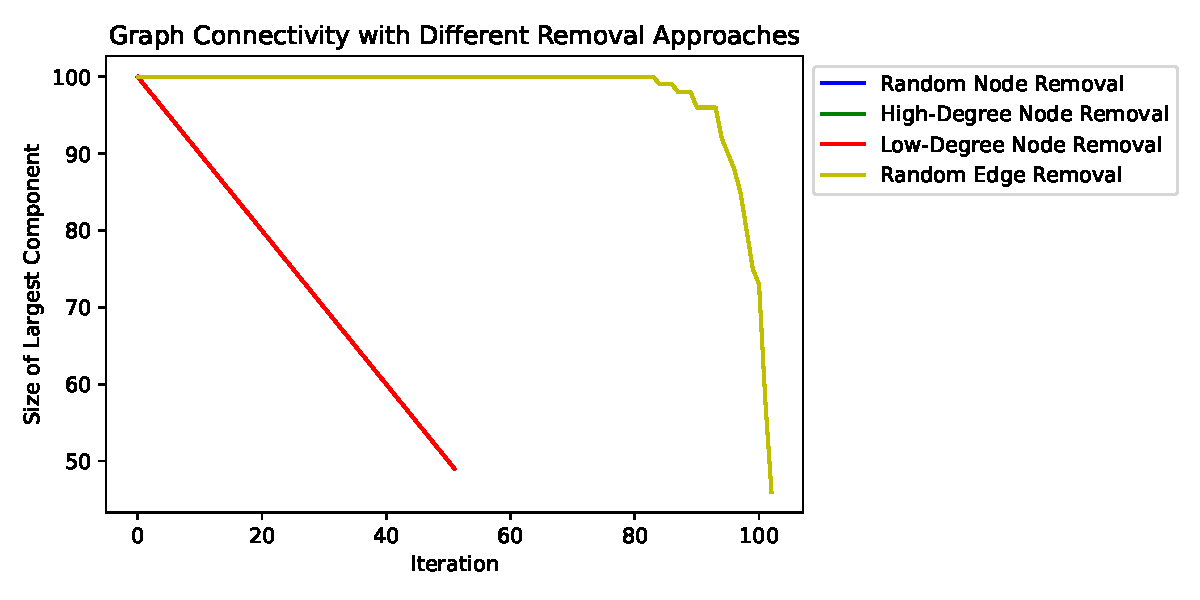
\includegraphics[width=1\linewidth]{random_network_connectivity_plot.pdf}
  \caption{Impact of Different Removal Strategies on Network Connectivity in an Erdős–Rényi Random Network}
  \label{fig:12.1}
\end{figure}

The most striking structural robustness occurred while randomly removing edges from the network. The network's structural integrity remained totally unaffected. The network showed the robustness up to 81 iterations (81\% of edge removal from the original network) with the largest component of 100 nodes (original generated network with no disconnected nodes).

The network demonstrated both resilience and robustness in response to each of the four distinct types of perturbations, highlighting its ability to adapt and maintain structural integrity under a variety of challenges. The random and uniform nature of these networks contributes to their resilience under different random node and edge removal strategies. Understanding these dynamics is essential for applications in diverse fields, from information dissemination to transportation systems, where random network structures often play a vital role.

The removal of random nodes from a scale-free network demonstrated remarkable resilience, as shown in Figure \ref{fig:12.2}. The network remained connected up to 21 iterations of random node removal, highlighting its robustness against the stochastic nature of this process. However, at the 35th iteration, the network faced again the disconnection, emphasizing its vulnerability to extensive random node removal.

Similarly, for the removal of high-degree nodes in a scale-free network, the network's vulnerability was evident. After just 4 iterations, the network gets disconnected, showcasing its susceptibility to the targeted removal of high-degree nodes. This disconnection resulted into 30 percent of the network as it's largest connected component after only 10 iterations.

\begin{figure}[t]
  \centering
  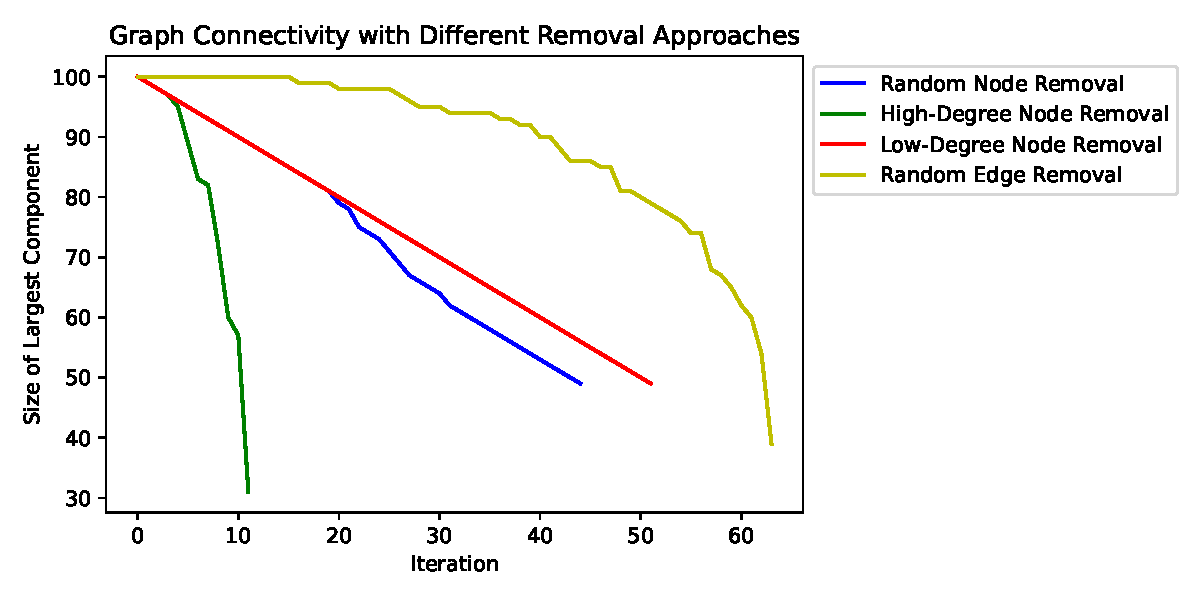
\includegraphics[width=1\linewidth]{scale_free_network_connectivity_plot.pdf}
  \caption{Impact of different removal strategies on network connectivity in a Barabási-Albert scale-free network}
  \label{fig:12.2}
\end{figure}

When subject to random edge removal, a scale-free network displayed moderate resilience. It maintained connectivity up to the 15th iteration of edge removal, highlighting its ability to adapt and stay intact to some extent under this perturbation.

Conversely, a scale-free network exhibited robustness in response to low-degree node removal. The network remained connected and adaptive, demonstrating its capacity to withstand the perturbation without significant structural impact.

These findings emphasize the behavior of scale-free networks under different perturbations and emphasize the importance of understanding their vulnerabilities and strengths in real-world applications.

In the case of random node removal within a small-world network, see Figure \ref{fig:12.3}, the network displayed moderate resilience to 27 iterations before facing disconnection.

When subjected to high-degree node removal, a small-world network demonstrated vulnerability, with disconnection occurring after 16 iterations. However, the network's susceptibility became apparent as early as 25 iterations, with almost a 50 percent reduction in its original size, highlighting the consequences of high-degree node removal. Conversely, low-degree node removal posed no threat to a small-world network's robustness. It remained connected throughout the removal process, even as 50 percent of the random nodes were removed, demonstrating its remarkable structural integrity.

\begin{figure}[t]
  \centering
  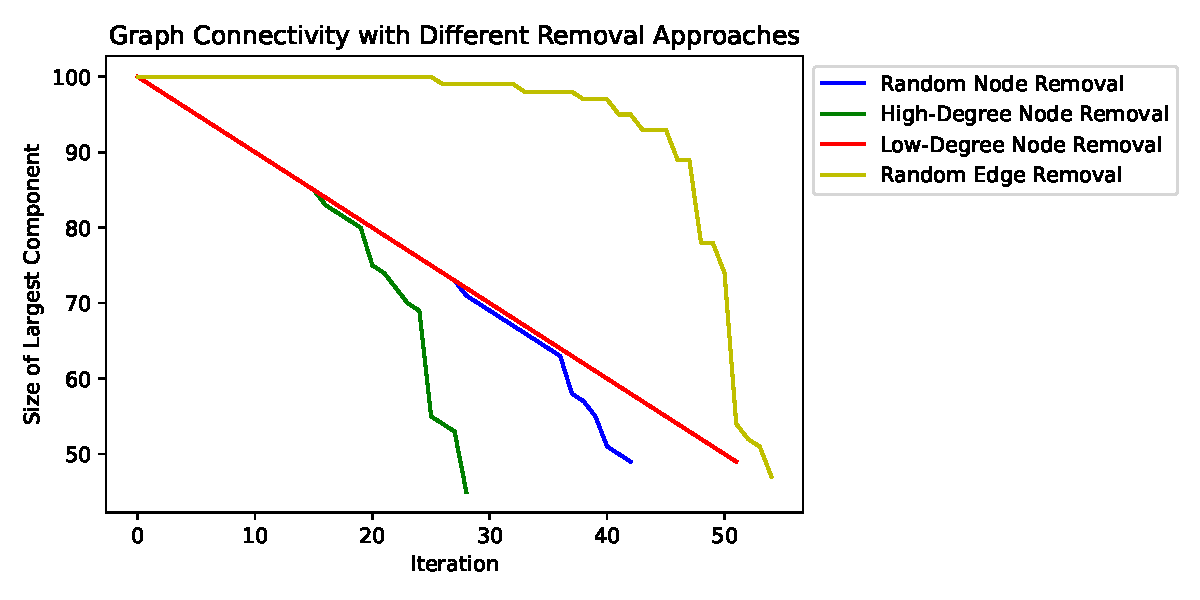
\includegraphics[width=1\linewidth]{small_world_network_connectivity_plot.pdf}
  \caption{Impact of Different Removal Strategies on Network Connectivity in a Watts-Strogatz Small-World Network}
  \label{fig:12.3}
\end{figure}

In the analysis of random edge removal in a small-world network, the network showed moderate resilient upto around 25\% of random edge removal but around 45th iteration, the network faced a significant drop, going from a 90 percent largest connected component to a 50 percent largest connected component. This dynamic response suggests that the network initially demonstrated the capability to adjust and maintain its connectivity in response to these random edge removal. However, as the edge removal increased, the network eventually reached a point where it could no longer adapt effectively and started to break down and lose its resilience.

These observations emphasize the behavior of small-world networks under various perturbation scenarios and underscore the importance of understanding their vulnerabilities and strengths in practical applications.

\subsection{Change in Network Structure}

In this subsection, we explore the impact of the node and edge removal strategies on the structure of the complex networks. We conducted a series of experiments to assess how the network's degree distribution evolves as we apply various removal strategies. These experiments were conducted on the same three types of random, scale-free, and small-world networks with the same parameters as discussed before in the methodology. Also, the same removal strategies included high-degree node removal, low-degree node removal, random node removal, and random edge removal and the removal percentage from 5\% to 25\%. By conducting these experiments on different network types, we aimed to gain insights into how each removal strategy influenced the degree frequency distribution of the network and, consequently, the overall network structure. From plot figures, the degree distribution plot where each plot illustrates a distinct removal strategy, and each color line represents the degree distribution in the corresponding network before and after a range of removal percentages. We used Non-parametric Kolmogorov-Smirnov (K-S) and Cramér-von Mises (CvM) tests with a significance level of 0.05 to statistically evaluate these changes.

\subsubsection{Impact of removal strategies on Random Network}

The frequency distribution plots of a random network before and after high-degree nodes removed are displayed in Figure \ref{fig:13.1}. The results of the high-degree node removal strategy are summarized in Table \ref{table:high_degree_node_removal}. The CvM and K-S statistics show a significant increase in the proportion of node removal. The CvM statistics consistently deviate from the original degree distribution, rising from 0.8888 at 5\% removal to 11.0364 at 25\% removal. The CvM statistics' p-values correspondingly decreased, signifying a significant deviation from the original distribution. Similar trends can be seen in the K-S statistics, which rise from 0.1984 at 5\% removal to 0.79 at 25\% reduction. The corresponding K-S test p-values similarly decreased to zero, confirming the significant effect of removing high-degree nodes on the degree distribution of the network. Based on these findings, the null hypothesis which states that the degree distribution of a random network is the same before and after a removal of high-degree nodes can be rejected.

\begin{figure}[t]
  \centering
  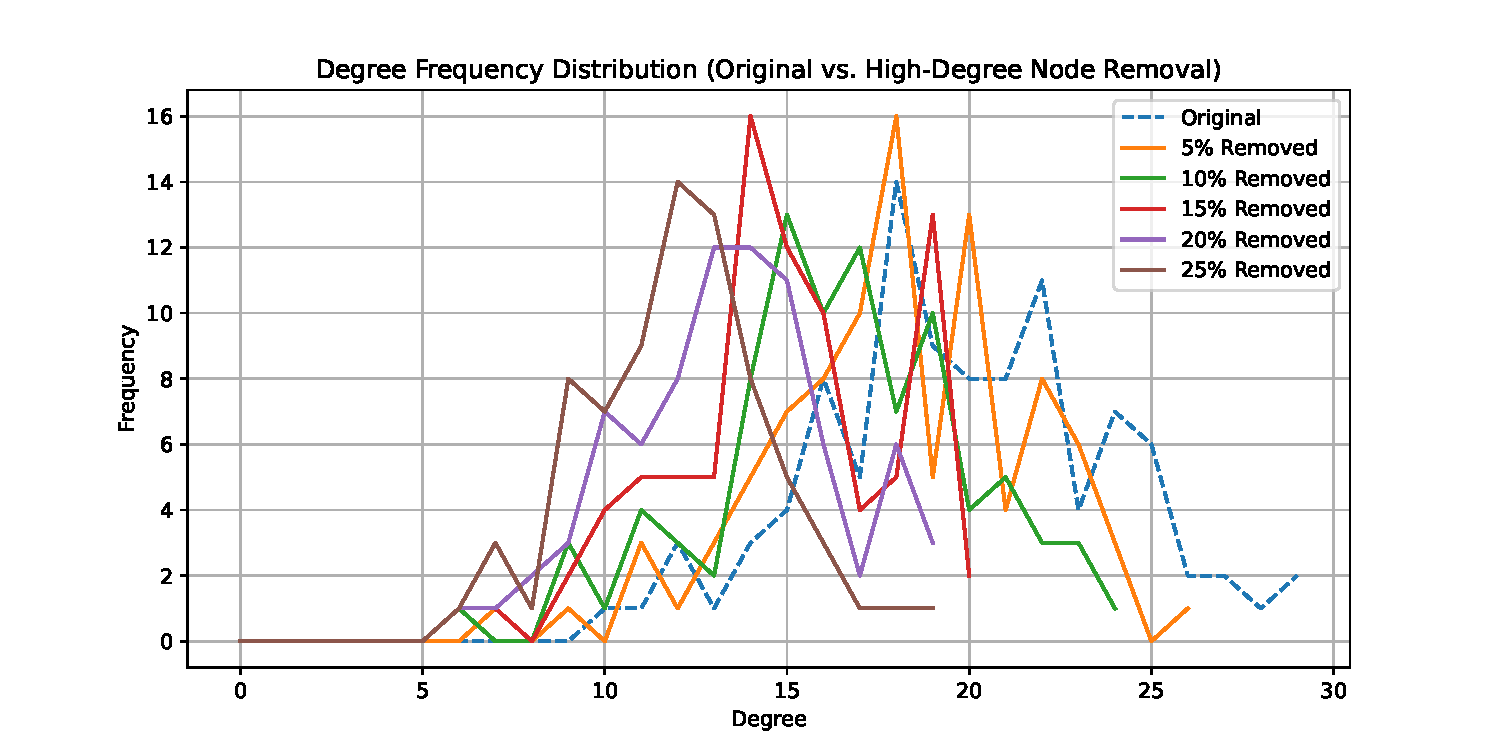
\includegraphics[width=1.1\linewidth]{random_network_frequency_distribution_plot_High-Degree Node Removal.pdf}
  \caption{Degree Frequency Distribution in Erdős–Rényi Random Network at different percentages of High-Degree Node Removal}
  \label{fig:13.1}
\end{figure}


The frequency distribution plots of a random network before and after the removal of low-degree nodes are shown in Figure \ref{fig:13.2}. Table \ref{table:low_degree_node_removal} provides an overview of the low-degree node removal strategy's results. As the percentage of nodes removed increases from 5\% to 25\%, there is a small but noticeable change in the degree distribution plot. This change is reflected in both the CvM and K-S statistics, which increase with increasing node removal. The decreasing p-values associated with the CvM and K-S statistics demonstrate that the observed changes in the degree distribution are statistically significant. As expected, the CvM test is more sensitive to the long tail of the plot than the K-S test. Given the importance of the long tail in network analysis, we can reject the hypothesis that the degree distribution remains unchanged even after removing 15\% of low-degree nodes.

\begin{figure}[t]
  \centering
  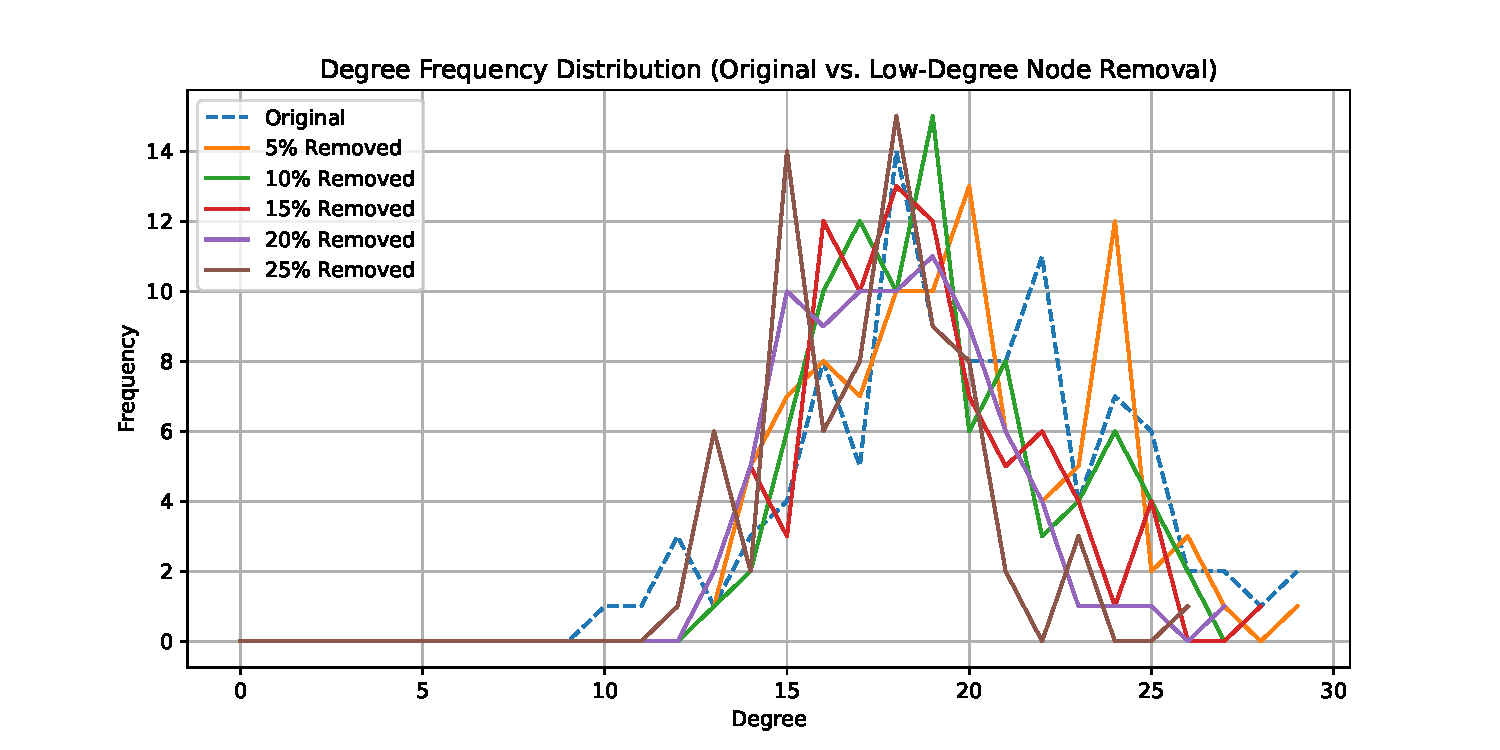
\includegraphics[width = 1.1\linewidth]{random_network_frequency_distribution_plot_Low-Degree Node Removal.pdf}
  \caption{Degree Frequency Distribution in Erdős–Rényi Random Network at different percentages of Low-Degree Node Removal}
  \label{fig:13.2}
\end{figure}

The results of the random node removal method are displayed in the frequency distribution plot (see Figure \ref{fig:13.3} and Table \ref{table:random_node_removal}). At 5\% removal, the CvM statistics show a slight increase to 0.1355, with a p-value of 0.4404, indicating no significant departure from the original distribution. However, as the percentage of nodes removed increases, the CvM statistics rise notably, reaching 5.5217 at 25\% removal, accompanied by a very low p-value. The K-S statistics also demonstrate a progressive increase, from 0.0826 at 5\% removal to 0.54 at 25\% removal, with corresponding p-values diminishing significantly, reinforcing the significant deviation from the original distribution. By combining the results, we fail to reject the null hypothesis for the removal of 5\% of random nodes, but we reject it for the remaining removal percentages. 

\begin{figure}[t]
  \centering
  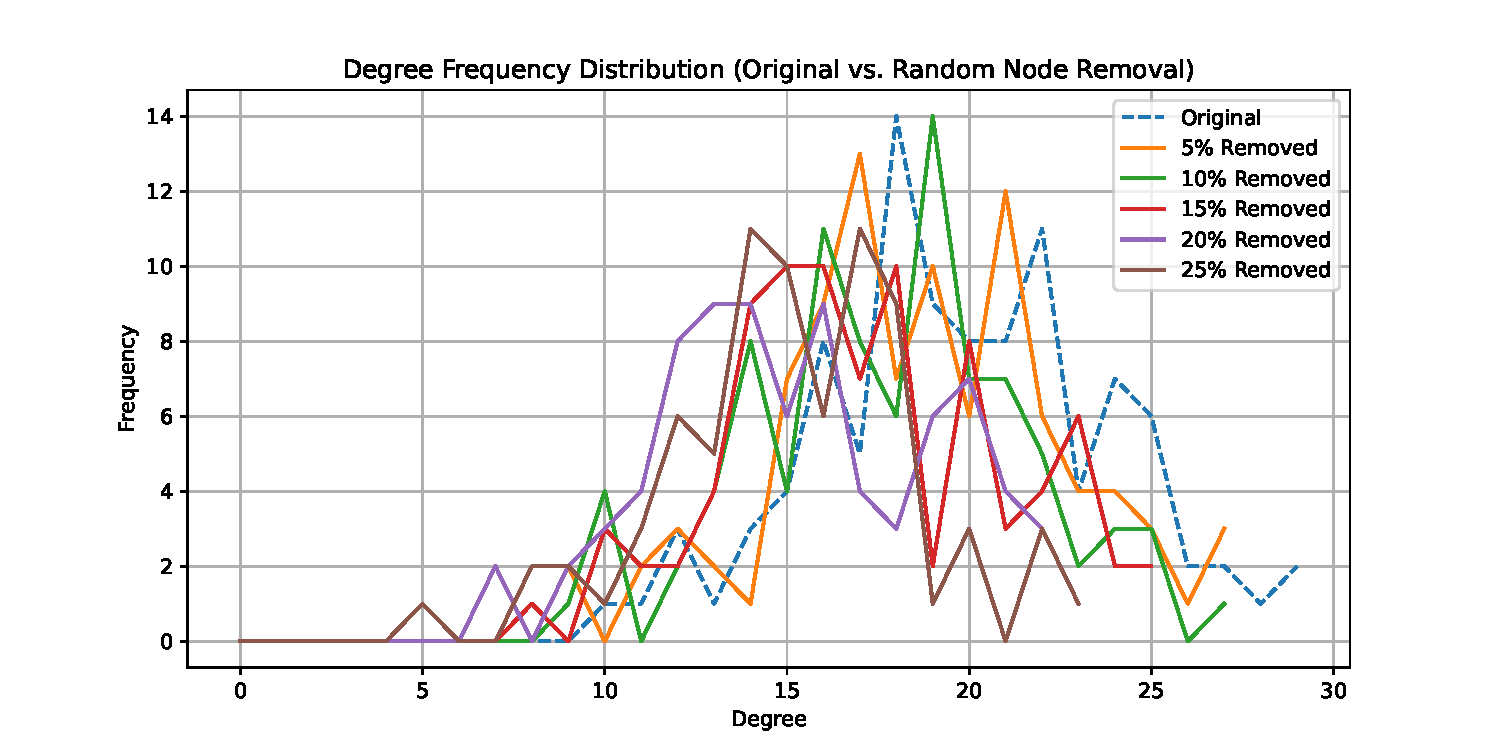
\includegraphics[width = 1.1\linewidth]{random_network_frequency_distribution_plot_Random Node Removal.pdf}
  \caption{Degree Frequency Distribution in Erdős–Rényi Random Network at different percentages of Random Node Removal.}
  \label{fig:13.3}
\end{figure}


\begin{figure}[t]
  \centering
  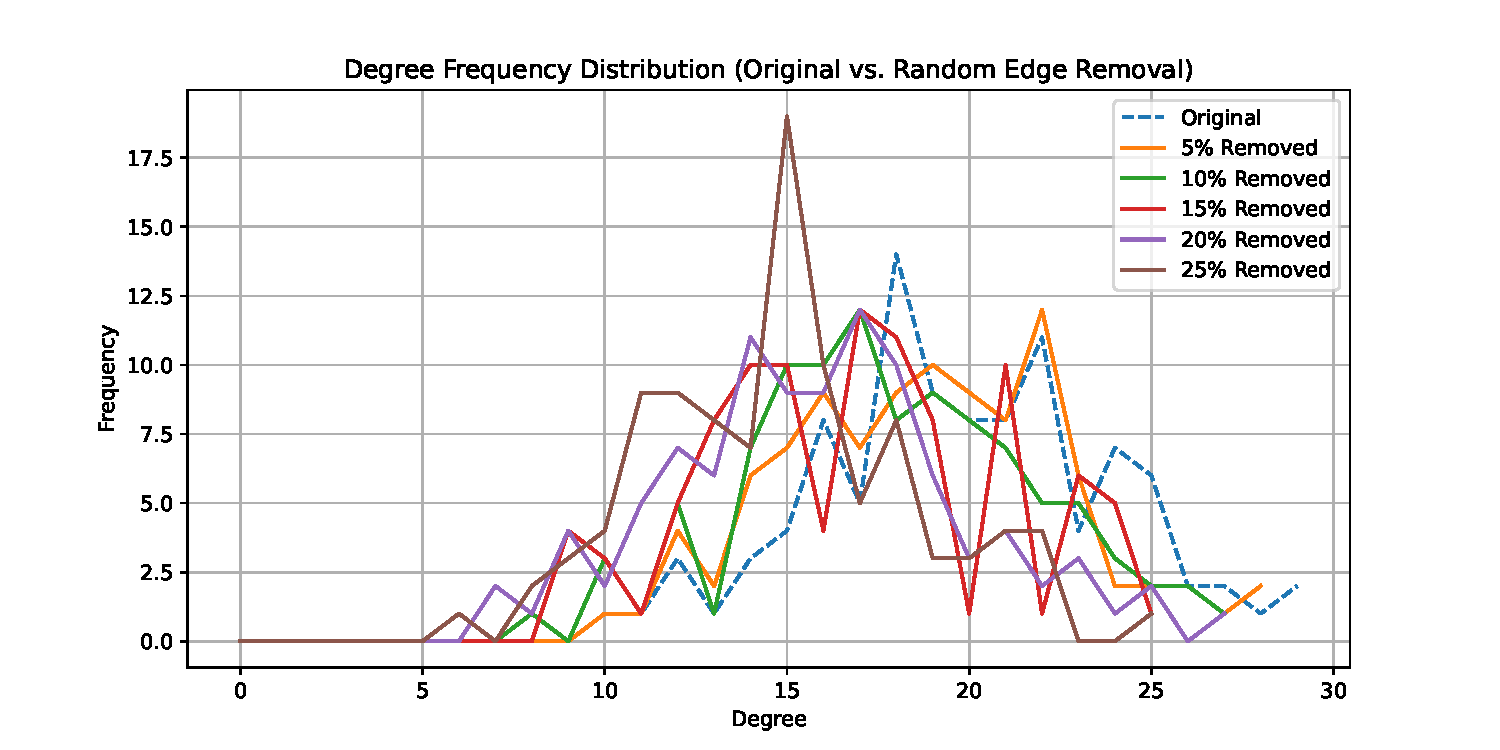
\includegraphics[width=1.1\linewidth]{random_network_frequency_distribution_plot_Random Edge Removal.pdf}
  \caption{Degree Frequency Distribution in Erdős–Rényi Random Network at different percentages of Random Edge Removal}
  \label{fig:13.4}
\end{figure}

The results of the random edge removal strategy, and frequency distribution plot are shown in Figure \ref{fig:13.4} and Table \ref{table:random_edge_removal} respectively. The CvM statistics increase from 0.2962 at 5\% removal with a p-value of 0.1390 to 6.0382 at 25\% removal with an extremely low p-value, indicating the statistical significance of structure change. The K-S statistics also show a progressive rise, from 0.12 at 5\% removal with a p-value of 0.4695 to 0.5 at 25\% removal with a very low p-value. The results of this study indicate how removing more than 5\% of random edges significantly affects the degree distribution, causing a noticeable and statistically significant deviation from the original distribution. Consequently, for the remaining removal percentages, we reject the null hypothesis.

\subsubsection{Impact of removal strategies on Scale-free Network}

The results of the high-degree node removal strategy in a scale-free network are the frequency distribution plots in Figure \ref{fig:14.1} and associated statistical test results in Table \ref{table:high_degree_node_removal_2}. The CvM statistics exhibit a significant increase, from 2.0114 at 5\% removal to 10.1317 at 25\% removal, with very low p-values consistently indicating statistical significance. Similar gradual changes are also shown by the K-S statistics, which indicate a significant shift in the degree distribution. These findings show the substantial impact of even 5\% of high-degree node removal on altering the network's degree distribution in a scale-free network. Hence, we reject the null hypothesis for each removal percentage.

\begin{figure}[t]
  \centering
  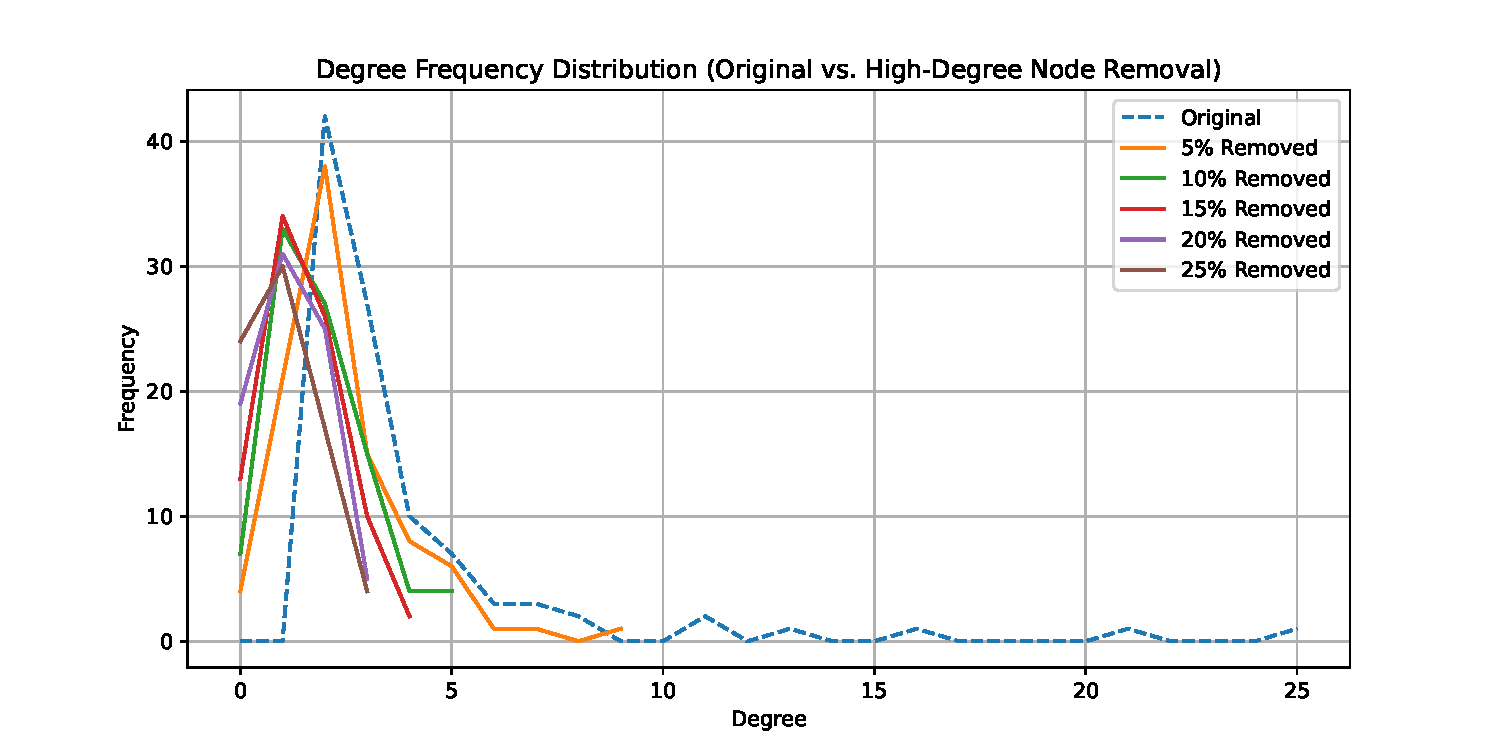
\includegraphics[width=1.1\linewidth]{scale_free_network_frequency_distribution_plot_High-Degree Node Removal.pdf}
  \caption{Degree Frequency Distribution in Barabási-Albert Scale-Free Network at different percentages of High-Degree Node Removal}
  \label{fig:14.1}
\end{figure}


The results from the low-degree node removal strategy in a scale-free network, the frequency distribution plot shown in Figure \ref{fig:14.2}, indicate a relatively mild impact on the degree distribution, the associated statistical results are presented in Table \ref{table:low_degree_node_removal_2}. The CvM statistics display a gradual increase from 0.0241 at 5\% removal to 0.2861 at 25\% removal, with p-values consistently higher than the significance value 0.05, suggesting no statistically significant deviation from the original distribution. Alongside, the K-S test demonstrates similar results, with the p-value higher than the significance value of 0.05 for all removal percentages. This suggests that removing low-degree nodes has a limited effect on the degree distribution in a scale-free network. Consequently, we fail to reject the null hypothesis.

\begin{figure}[t]
  \centering
  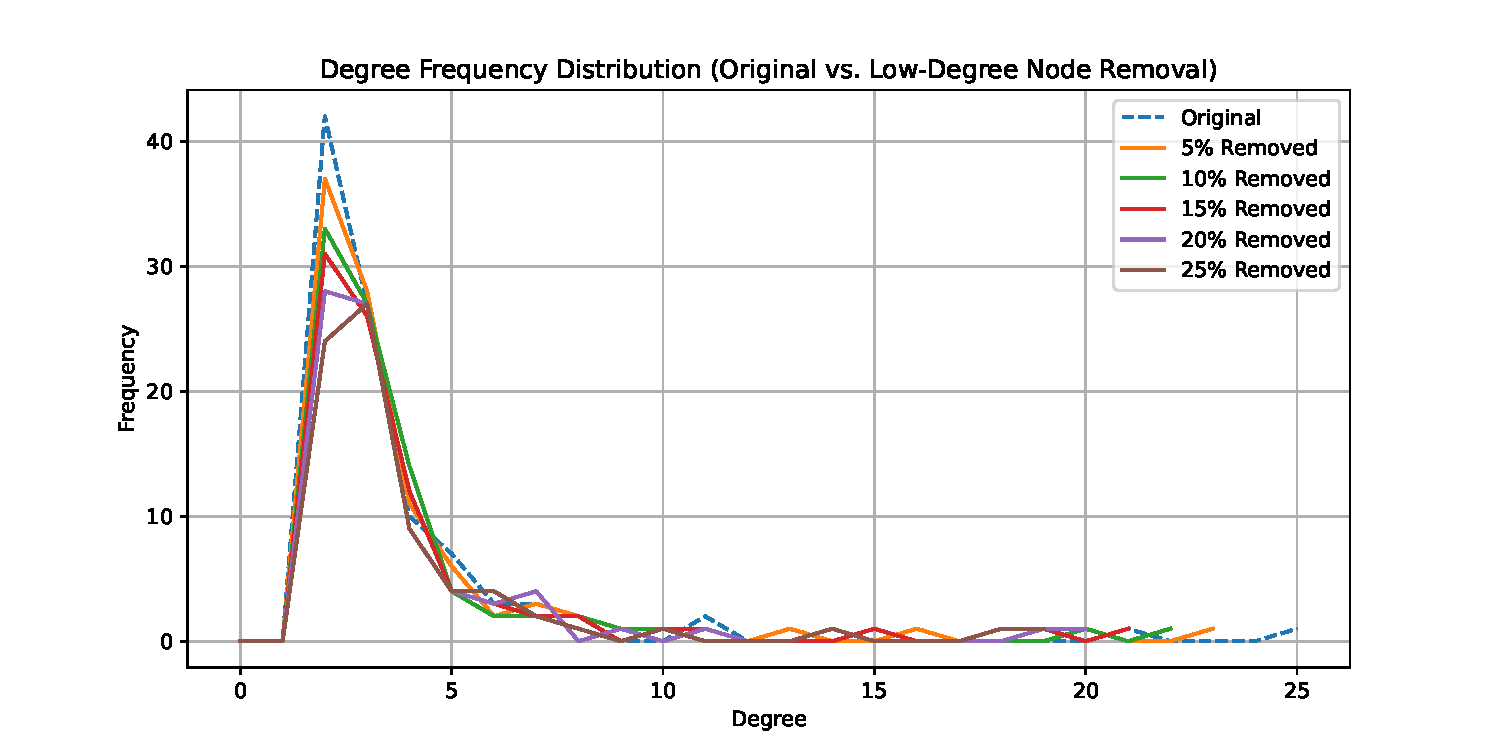
\includegraphics[width=1.1\linewidth]{scale_free_network_frequency_distribution_plot_Low-Degree Node Removal.pdf}
  \caption{Degree Frequency Distribution in Barabási-Albert Scale-Free Network at different percentages of Low-Degree Node Removal}
  \label{fig:14.2}
\end{figure}

The results from a scale-free network, as the frequency distribution plot shown in Figure \ref{fig:14.3} and the statistical results shown in Table \ref{table:random_node_removal_2}, indicate that random node removal has a minimal impact on the degree distribution for removal percentages up to 15\%. The CvM statistics show deviations, with p-values remaining lesser than the significance value of 0.05. However, at 20\% and 25\% removal, a more noticeable shift is observed, with CvM statistics reaching 0.5121 and 1.3568, respectively, and p-values dropping to 0.0371 and 0.0004, indicating a statistically significant deviation from the original distribution. Additionally, the K-S test also showed similar results up to 20\% of random node removal with K-S statistics 0.15 and p-value 0.2456. This suggests that the effect of random node removal on the degree distribution becomes more pronounced as the percentage of removed nodes increases, leading to the rejection of the null hypothesis for  25\% of random node removal.

\begin{figure}[t]
  \centering
  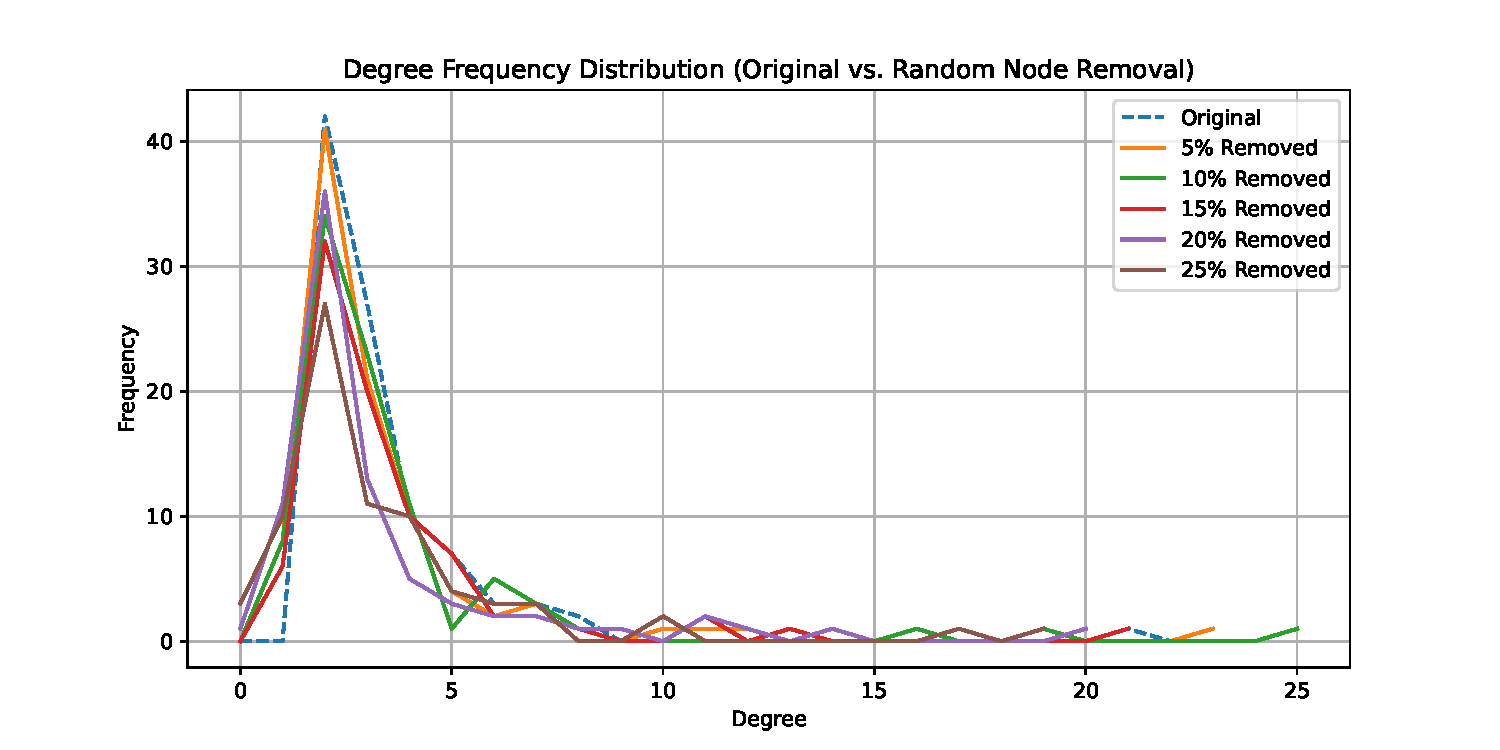
\includegraphics[width=1.1\linewidth]{scale_free_network_frequency_distribution_plot_Random Node Removal.pdf}
  \caption{Degree Frequency Distribution in Barabási-Albert Scale-Free Network at different percentages of Random Node Removal}
  \label{fig:14.3}
\end{figure}

The results of a scale-free network after random edge removal are illustrated in Figure \ref{fig:14.4} and associated statistical results in Table \ref{table:random_edge_removal_2}. The CvM statistics progressively increase from 0.0380 at 5\% removal to 1.3194 at 25\% removal, with p-values decreasing significantly from 15\% removal. Simultaneously, the K-S test provided similar results with a p-value below the significant value of 0.05 from 20\% removal, further supporting the significant deviation from the original distribution. Here, we reject the null hypothesis at 20\% and 25\% removal of random edges.

\begin{figure}[t]
  \centering
  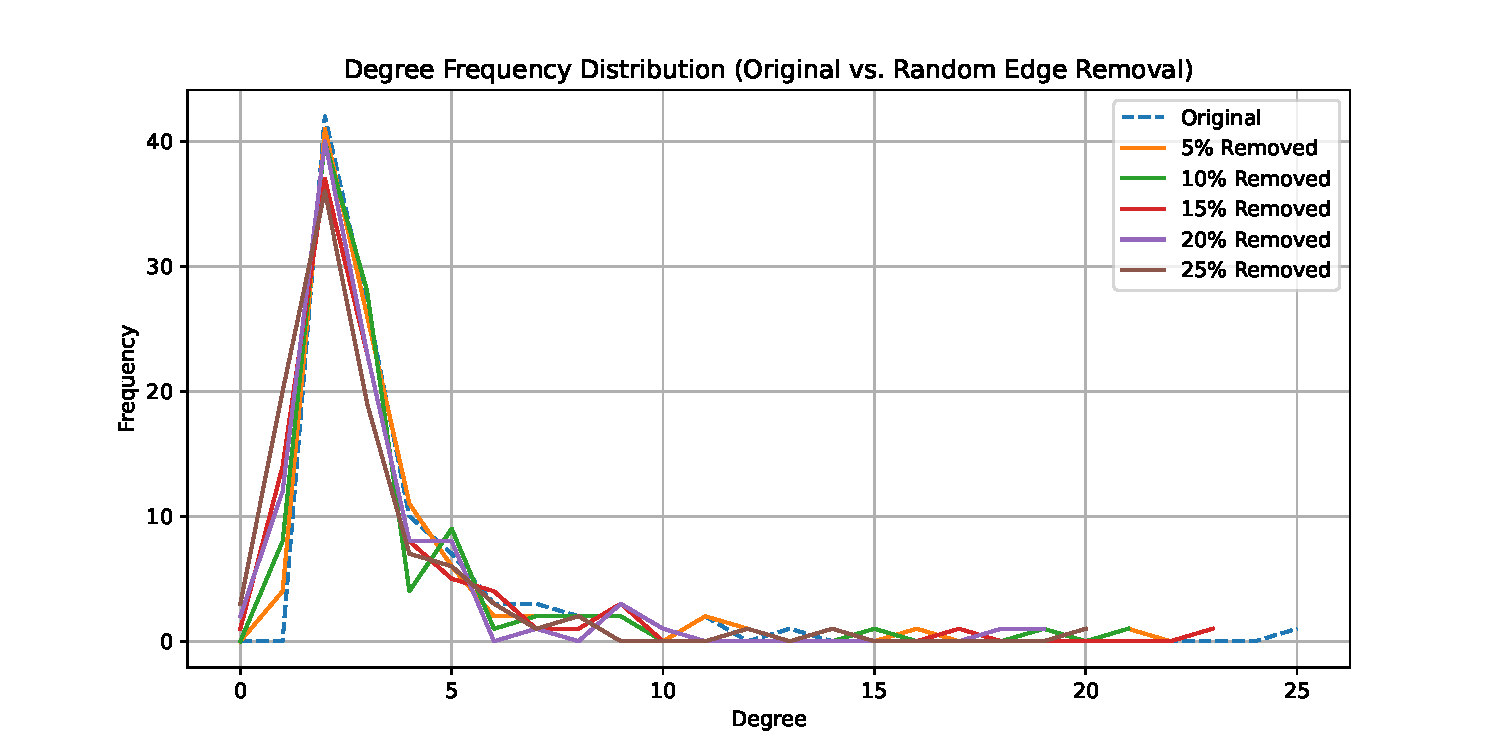
\includegraphics[width=1.1\linewidth]{scale_free_network_frequency_distribution_plot_Random Edge Removal.pdf}
  \caption{Degree Frequency Distribution in Barabási-Albert Scale-Free Network at different percentages of Random Edge Removal}
  \label{fig:14.4}
\end{figure}

\subsubsection{Impact of removal strategies on Small-world Network}

The frequency distribution plots in Figure \ref{fig:15.1} shows the impact of high-degree node removal on the degree distribution of a small-world network. The associated statistical results are presented in Table \ref{table:high_degree_node_removal_3}. The CvM test is more sensitive to these changes, at 5\% removal, the CvM statistic is 0.5494 with a p-value of 0.0299, indicating a significant deviation from the original degree distribution. The K-S test, on the other hand, showed lower statistics and a p-value higher than the significance level of 0.05 for both 5\% and 10\% removal. However, after 10\% removal, the K-S test also indicated a significant deviation with a p-value lower than the significance level. This suggests that the CvM test is more sensitive to changes in the degree distribution of high-degree nodes so, we reject the null hypothesis at higher removal percentages including at 10\% removal of high-degree nodes.

\begin{figure}[t]
  \centering
  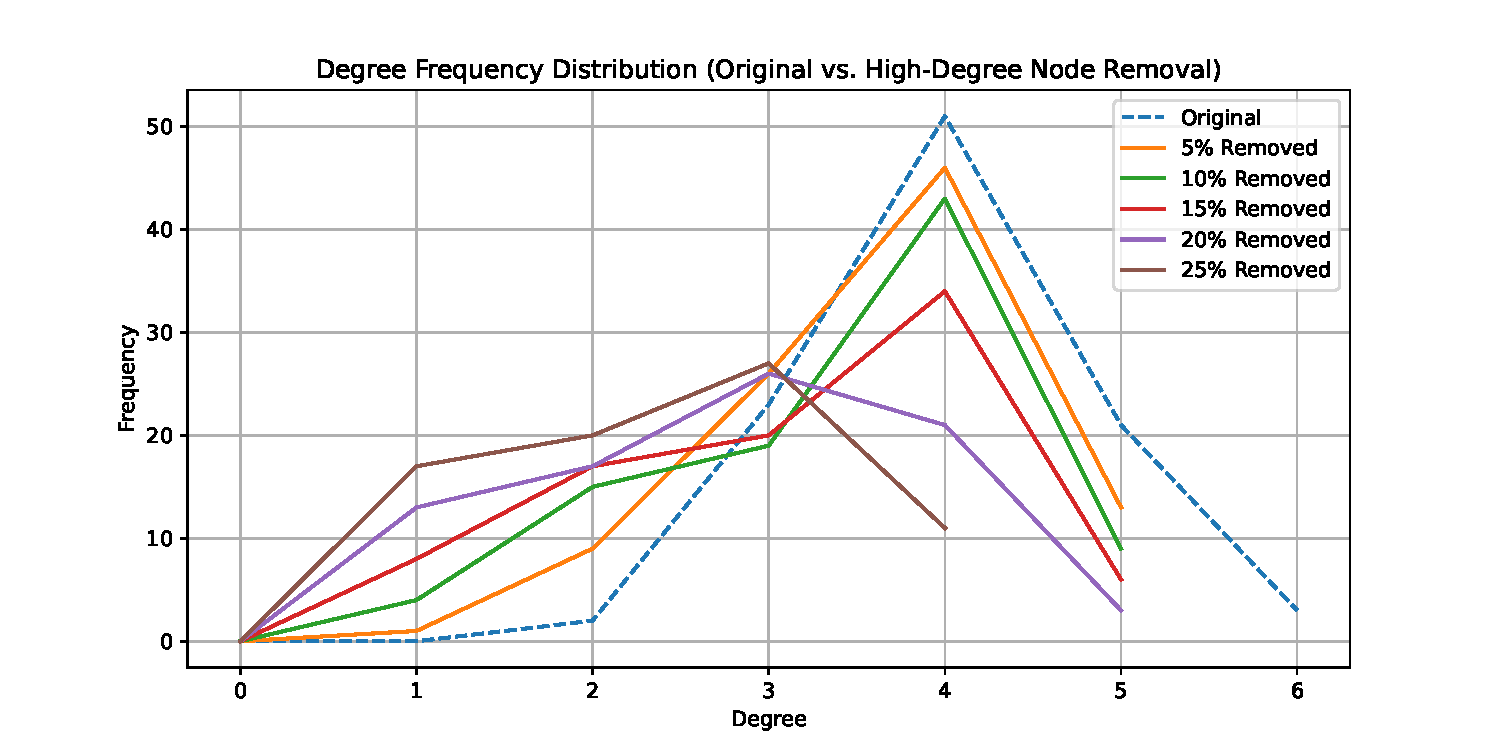
\includegraphics[width=1.1\linewidth]{small_world_network_frequency_distribution_plot_High-Degree Node Removal.pdf}
  \caption{Degree Frequency Distribution in Watts-Strogatz Small-World Network at different percentages of High-Degree Node Removal}
  \label{fig:15.1}
\end{figure}


Figure \ref{fig:15.2} visually represents the impact of the Low-Degree Node Removal strategy on a small-world network's degree distribution, with detailed statistical results presented in Table \ref{table:low_degree_node_removal_3}. Initially, at a 5\% removal rate, the CvM statistics of 0.0314 and a p-value of 0.9754 indicated no noteworthy deviation. However, as the removal percentage increased, statistical significance became apparent, with a CvM statistic of 0.9680 and a significantly low p-value of 0.0029 at 20\% removal, further decreasing at higher percentages. The corresponding K-S test at 20\% removal, featuring K-S statistics of 0.1750 and a p-value of 0.1172, suggests that low-degree node removal did impact the degree distribution, although the effect was not significant. A statistically significant shift in distribution was detected at 25\% removal, with K-S statistics of 0.2700 and a p-value of 0.0032. These findings demonstrate that the removal of low-degree nodes has a gradual impact on the degree distribution of a small-world network. Here, we reject the null hypothesis only at 25\% removal of low-degree nodes.

\begin{figure}[t]
  \centering
  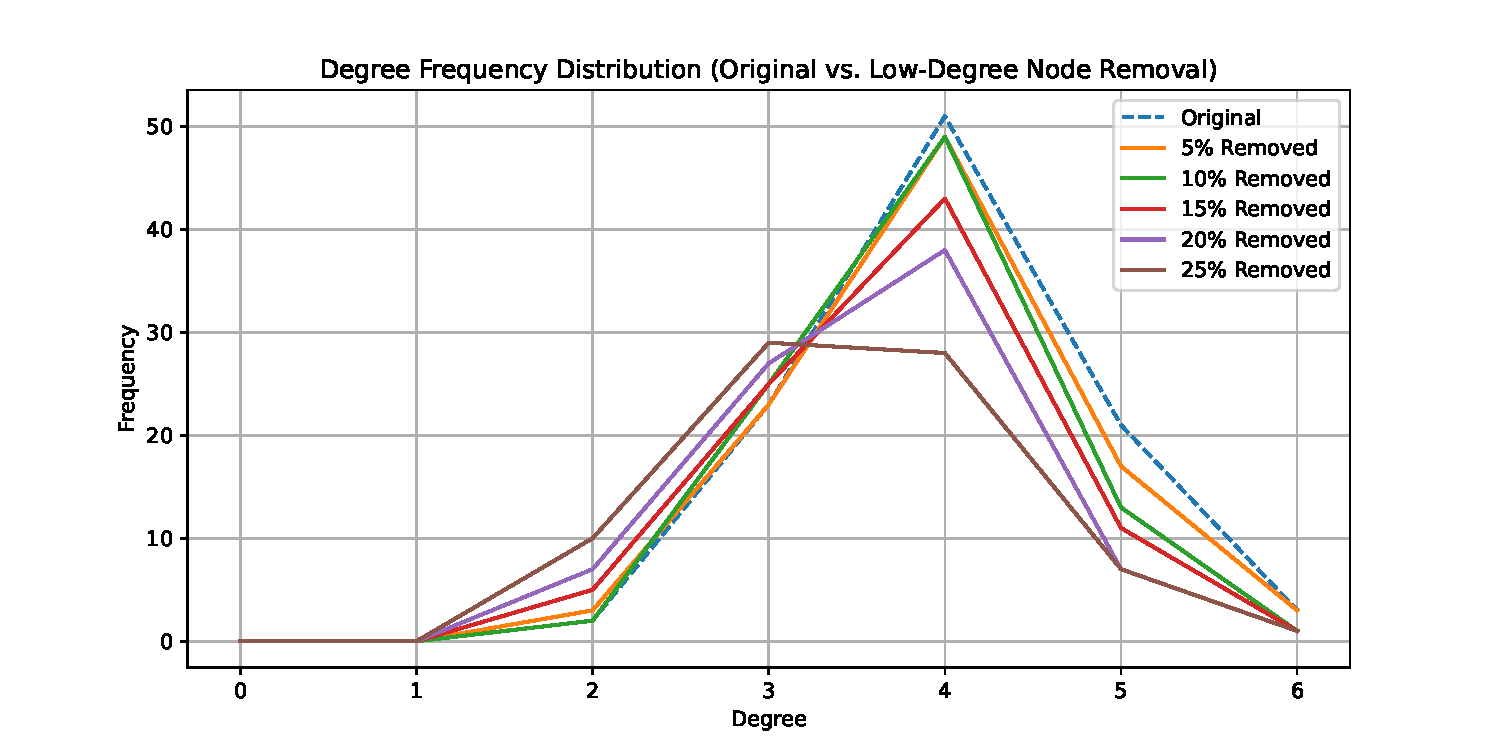
\includegraphics[width=1.1\linewidth]{small_world_network_frequency_distribution_plot_Low-Degree Node Removal.pdf}
  \caption{Degree Frequency Distribution in Watts-Strogatz Small-World Network at different percentages of Low-Degree Node Removal}
  \label{fig:15.2}
\end{figure}

The effect of the random node removal strategy on the degree distribution of a small-world network is presented in Figure \ref{fig:15.3} and the corresponding statistical results are presented in Table \ref{table:random_node_removal_3}. At 5\% removal, the CvM statistics of 0.2938 and a p-value of 0.1412 indicated no significant deviation from the original distribution. However, as removal percentages increased, we can see the statistical significance. Notably, at 15\% removal, a CvM statistic of 2.3229 and a very low p-value highlighted a substantial deviation from the original distribution. This was supported by the corresponding K-S statistic, which also increased to 0.3265 at 15\% removal, along with a p-value lower than the significance level of 0.05. The higher sensitivity of the CvM test to changes in the distribution of high-degree nodes suggests that the observed deviation is likely due to the removal of these nodes. So, We reject the null hypothesis for the higher percentage including 15\% removal of random nodes.

\begin{figure}[t]
  \centering
  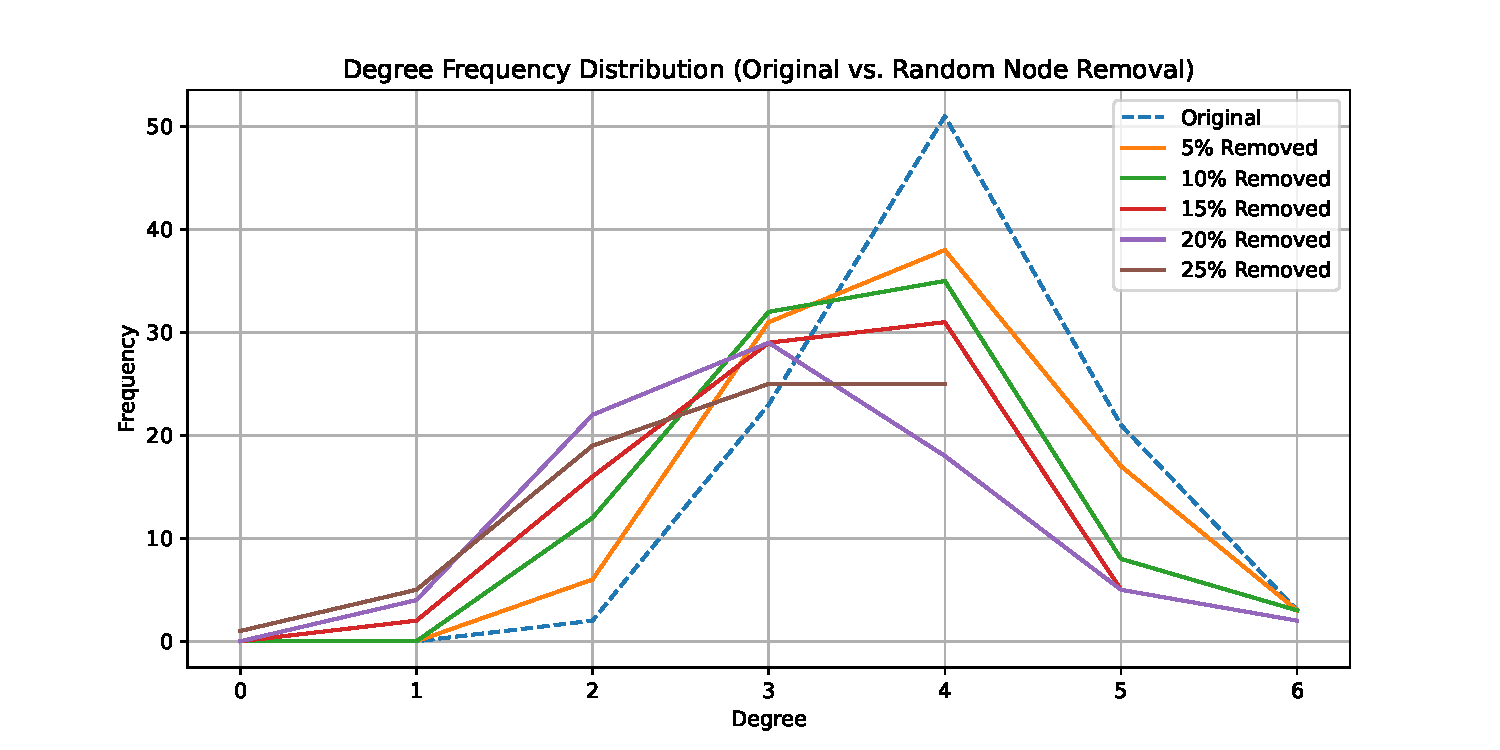
\includegraphics[width=1.1\linewidth]{small_world_network_frequency_distribution_plot_Random Node Removal.pdf}
  \caption{Degree Frequency Distribution in Watts-Strogatz Small-World Network at different percentages of Random Node Removal}
  \label{fig:15.3}
\end{figure}


In Figure \ref{fig:15.4}, we present the effects of random edge removal strategy on a small-world network's degree distribution and the associated statistical results are presented in Table \ref{table:random_edge_removal_3}. At 5\% removal, CvM statistic 0.2243 and K-S statistic 0.09 indicated no significant change, aligning with p-values of 0.2260 and 0.8154, respectively. However, at 10\% removal and higher removal percentages, both tests illustrated progressively significant deviations from the original distribution. By 25\% removal, the CvM p-value and K-S p-value became very low, indicating the strategy's significant impact on the network's structural integrity. From these results, we reject the hypothesis for higher removal percentages including 10\% removal of random edges.

\begin{figure}[t]
  \centering
  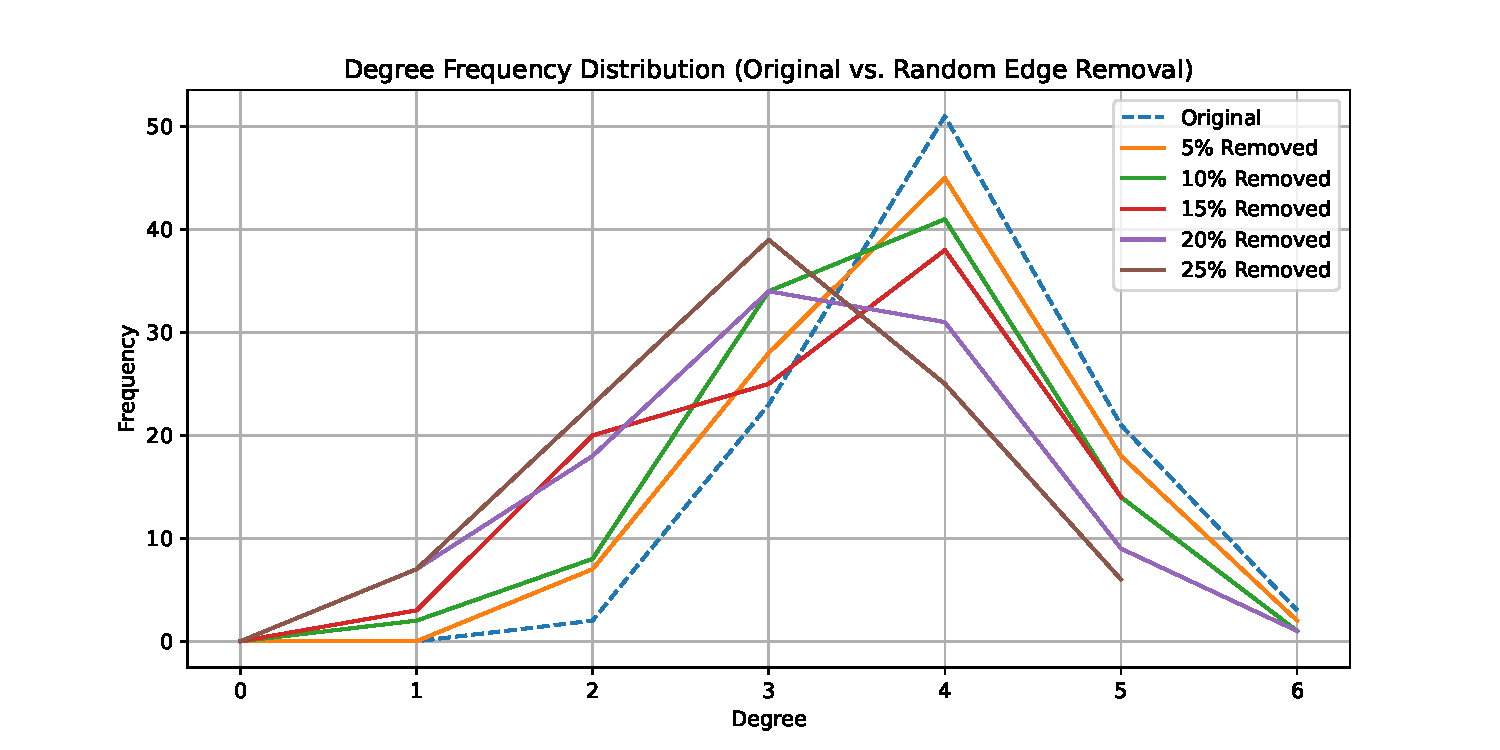
\includegraphics[width=1.1\linewidth]{small_world_network_frequency_distribution_plot_Random Edge Removal.pdf}
  \caption{Degree Frequency Distribution in Watts-Strogatz Small-World Network at different percentages of Random Edge Removal}
  \label{fig:15.4}
\end{figure}

\begin{table*}[h]
    \centering
    \caption{Erdős–Rényi Random Network: Statistical Test Results after High-Degree Node Removal}
    %\small % Reduce font size
    \begin{tabular}{|>{\raggedleft\arraybackslash}p{1.5cm}|>{\raggedleft\arraybackslash}p{2.5cm}|>{\raggedleft\arraybackslash}p{2.5cm}|>{\raggedleft\arraybackslash}p{2.5cm}|>{\raggedleft\arraybackslash}p{2.5cm}|}
        \hline
        \textbf{Percentage} & \textbf{CvM Statistic} & \textbf{P-Value (CvM)} & \textbf{K-S Statistic} & \textbf{P-Value (K-S)} \\ \hline
        5\% & 0.8888 & 0.0045 & 0.1984 & $3.60 \times 10^{-2}$ \\ \hline
        10\% & 3.0736 & $5.02 \times 10^{-8}$ & 0.3733 & $2.11 \times 10^{-6}$ \\ \hline
        15\% & 6.2458 & $1.97 \times 10^{-11}$ & 0.5076 & $2.46 \times 10^{-11}$ \\ \hline
        20\% & 8.9809 & $2.73 \times 10^{-10}$ & 0.6575 & $1.09 \times 10^{-18}$ \\ \hline
        25\% & 11.0364 & $2.53 \times 10^{-10}$ & 0.7900 & $4.36 \times 10^{-27}$ \\ \hline
    \end{tabular}
    \label{table:high_degree_node_removal}
%\end{table}

\vspace*{0.5cm}
% Low-Degree Node Removal Table
%\begin{table}[t]
    \centering
    \caption{Erdős–Rényi Random Network: Statistical Test Results after Low-Degree Node Removal}
    %\small % Reduce font size
    \begin{tabular}{|>{\raggedleft\arraybackslash}p{1.5cm}|>{\raggedleft\arraybackslash}p{2.5cm}|>{\raggedleft\arraybackslash}p{2.5cm}|>{\raggedleft\arraybackslash}p{2.5cm}|>{\raggedleft\arraybackslash}p{2.5cm}|}
        \hline
        \textbf{Percentage} & \textbf{CvM Statistic} & \textbf{P-Value (CvM)} & \textbf{K-S Statistic} & \textbf{P-Value (K-S)} \\ \hline
        5\% & 0.0599 & 0.8219 & 0.0721 & 0.9394 \\ \hline
        10\% & 0.2897 & 0.1451 & 0.1322 & 0.3430 \\ \hline
        15\% & 0.6399 & 0.0178 & 0.1829 & 0.0791 \\ \hline
        20\% & 1.2772 & 0.0006 & 0.2550 & 0.0051 \\ \hline
        25\% & 2.2123 & $4.16 \times 10^{-6}$ & 0.35 & $3.79 \times 10^{-5}$ \\ \hline
    \end{tabular}
    \label{table:low_degree_node_removal}
%\end{table}

\vspace*{0.5cm}
% Random Node Removal Table
%\begin{table}[t]
    \centering
    \caption{Erdős–Rényi Random Network: Statistical Test Results after Random Node Removal}
    %\small % Reduce font size
    \begin{tabular}{|>{\raggedleft\arraybackslash}p{1.5cm}|>{\raggedleft\arraybackslash}p{2.5cm}|>{\raggedleft\arraybackslash}p{2.5cm}|>{\raggedleft\arraybackslash}p{2.5cm}|>{\raggedleft\arraybackslash}p{2.5cm}|}
        \hline
        \textbf{Percentage} & \textbf{CvM Statistic} & \textbf{P-Value (CvM)} & \textbf{K-S Statistic} & \textbf{P-Value (K-S)} \\ \hline
        5\% & 0.1355 & 0.4404 & 0.0826 & 0.8563 \\ \hline
        10\% & 0.9319 & 0.0035 & 0.2 & 0.0383 \\ \hline
        15\% & 2.8869 & $1.30 \times 10^{-7}$ & 0.3518 & $1.42 \times 10^{-5}$ \\ \hline
        20\% & 3.4546 & $7.19 \times 10^{-9}$ & 0.4025 & $6.09 \times 10^{-7}$ \\ \hline
        25\% & 5.5217 & $3.51 \times 10^{-10}$ & 0.54 & $5.85 \times 10^{-12}$ \\ \hline
    \end{tabular}
    \label{table:random_node_removal}
%\end{table}

\vspace*{0.5cm}
% Random Edge Removal Table
%\begin{table}[t]
    \centering
    \caption{Erdős–Rényi Random Network: Statistical Test Results after Random Edge Removal}
    %\small % Reduce font size
    \begin{tabular}{|>{\raggedleft\arraybackslash}p{1.5cm}|>{\raggedleft\arraybackslash}p{2.5cm}|>{\raggedleft\arraybackslash}p{2.5cm}|>{\raggedleft\arraybackslash}p{2.5cm}|>{\raggedleft\arraybackslash}p{2.5cm}|}
        \hline
        \textbf{Percentage} & \textbf{CvM Statistic} & \textbf{P-Value (CvM)} & \textbf{K-S Statistic} & \textbf{P-Value (K-S)} \\ \hline
        5\% & 0.2962 & 0.1390 & 0.12 & 0.4695 \\ \hline
        10\% & 1.1043 & 0.0014 & 0.23 & 0.0099 \\ \hline
        15\% & 2.5327 & $8.03 \times 10^{-7}$ & 0.33 & $3.21 \times 10^{-5}$ \\ \hline
        20\% & 4.1507 & $2.12 \times 10^{-10}$ & 0.43 & $1.12 \times 10^{-8}$ \\ \hline
        25\% & 6.0382 & $9.28 \times 10^{-12}$ & 0.5 & $1.00 \times 10^{-11}$ \\ \hline
    \end{tabular}
    \label{table:random_edge_removal}
%\end{table*}

\vspace*{0.5cm}
% High-Degree Node Removal Table for Barabási-Albert Scale-Free Network
%\begin{table*}[h]
    \centering
    \caption{Barabási-Albert Scale-Free Network: Statistical Test Results after High-Degree Node Removal}
    %\scriptsize % Reduce font size
    \begin{tabular}{|>{\raggedleft\arraybackslash}p{1.5cm}|>{\raggedleft\arraybackslash}p{2.5cm}|>{\raggedleft\arraybackslash}p{2.5cm}|>{\raggedleft\arraybackslash}p{2.5cm}|>{\raggedleft\arraybackslash}p{2.5cm}|}
        \hline
        \textbf{Percentage} & \textbf{CvM Statistic} & \textbf{P-Value (CvM)} & \textbf{K-S Statistic} & \textbf{P-Value (K-S)} \\ \hline
        5\% & 2.0114 & $1.18 \times 10^{-5}$ & 0.2632 & $1.78 \times 10^{-3}$ \\ \hline
        10\% & 4.5115 & $3.88 \times 10^{-11}$ & 0.4444 & $5.88 \times 10^{-9}$ \\ \hline
        15\% & 7.2186 & $3.69 \times 10^{-10}$ & 0.5529 & $1.79 \times 10^{-13}$ \\ \hline
        20\% & 9.0646 & $3.25 \times 10^{-10}$ & 0.6250 & $8.85 \times 10^{-17}$ \\ \hline
        25\% & 10.1317 & $2.38 \times 10^{-9}$ & 0.7200 & $5.89 \times 10^{-22}$ \\ \hline
    \end{tabular}
    \label{table:high_degree_node_removal_2}
%\end{table}

\vspace*{0.5cm}

% Low-Degree Node Removal Table for Barabási-Albert Scale-Free Network
%\begin{table}[t]
    \centering
    \caption{Barabási-Albert Scale-Free Network: Statistical Test Results after Low-Degree Node Removal}
    %\scriptsize % Reduce font size
    \begin{tabular}{|>{\raggedleft\arraybackslash}p{1.5cm}|>{\raggedleft\arraybackslash}p{2.5cm}|>{\raggedleft\arraybackslash}p{2.5cm}|>{\raggedleft\arraybackslash}p{2.5cm}|>{\raggedleft\arraybackslash}p{2.5cm}|}
        \hline
        \textbf{Percentage} & \textbf{CvM Stat.} & \textbf{P-Value (CvM)} & \textbf{K-S Stat.} & \textbf{P-Value (K-S)} \\ \hline
        5\% & 0.0241 & 0.9934 & 0.0305 & 0.9999 \\ \hline
        10\% & 0.0840 & 0.6754 & 0.0533 & 0.9978 \\ \hline
        15\% & 0.1083 & 0.5505 & 0.0553 & 0.9969 \\ \hline
        20\% & 0.1637 & 0.3528 & 0.0700 & 0.9707 \\ \hline
        25\% & 0.2861 & 0.1485 & 0.1000 & 0.7523 \\ \hline
    \end{tabular}
    \label{table:low_degree_node_removal_2}
\end{table*}

\vspace*{0.5cm}

% Random Node Removal Table for Barabási-Albert Scale-Free Network
\begin{table*}[t]
    \centering
    \caption{Barabási-Albert Scale-Free Network: Statistical Test Results after Random Node Removal}
    \small % Reduce font size
    \begin{tabular}{|>{\raggedleft\arraybackslash}p{1.5cm}|>{\raggedleft\arraybackslash}p{2.5cm}|>{\raggedleft\arraybackslash}p{2.5cm}|>{\raggedleft\arraybackslash}p{2.5cm}|>{\raggedleft\arraybackslash}p{2.5cm}|}
        \hline
        \textbf{Percentage} & \textbf{CvM Statistic} & \textbf{P-Value (CvM)} & \textbf{K-S Statistic} & \textbf{P-Value (K-S)} \\ \hline
        5\% & 0.0363 & 0.9564 & 0.0326 & 0.9999 \\ \hline
        10\% & 0.1855 & 0.2993 & 0.0889 & 0.8092 \\ \hline
        15\% & 0.2839 & 0.1508 & 0.0976 & 0.7269 \\ \hline
        20\% & 0.5121 & 0.0371 & 0.1500 & 0.2456 \\ \hline
        25\% & 1.3568 & 0.0004 & 0.2133 & 0.0354 \\ \hline
    \end{tabular}
    \label{table:random_node_removal_2}
%\end{table*}

\vspace*{0.5cm}

% Random Edge Removal Table for Barabási-Albert Scale-Free Network
%\begin{table*}[t]
    \centering
    \caption{Barabási-Albert Scale-Free Network: Statistical Test Results after Random Edge Removal}
    \small % Reduce font size
    \begin{tabular}{|>{\raggedleft\arraybackslash}p{1.5cm}|>{\raggedleft\arraybackslash}p{2.5cm}|>{\raggedleft\arraybackslash}p{2.5cm}|>{\raggedleft\arraybackslash}p{2.5cm}|>{\raggedleft\arraybackslash}p{2.5cm}|}
        \hline
        \textbf{Percentage} & \textbf{CvM Statistic} & \textbf{P-Value (CvM)} & \textbf{K-S Statistic} & \textbf{P-Value (K-S)} \\ \hline
        5\% & 0.0380 & 0.9488 & 0.0500 & 0.9997 \\ \hline
        10\% & 0.1921 & 0.2849 & 0.0800 & 0.9084 \\ \hline
        15\% & 0.4865 & 0.0431 & 0.1500 & 0.2112 \\ \hline
        20\% & 0.7992 & 0.0073 & 0.2100 & 0.0241 \\ \hline
        25\% & 1.3194 & $4.42 \times 10^{-4}$ & 0.2100 & 0.0241 \\ \hline
    \end{tabular}
    \label{table:random_edge_removal_2}
%\end{table*}

\vspace*{0.5cm}

% High-Degree Node Removal Table for Watts-Strogatz Small-World Network
%\begin{table*}[h]
    \centering
    \caption{Watts-Strogatz Small-World Network: Statistical Test Results after High-Degree Node Removal}
    %\small % Reduce font size
    \begin{tabular}{|>{\raggedleft\arraybackslash}p{1.5cm}|>{\raggedleft\arraybackslash}p{2.5cm}|>{\raggedleft\arraybackslash}p{2.5cm}|>{\raggedleft\arraybackslash}p{2.5cm}|>{\raggedleft\arraybackslash}p{2.5cm}|}
        \hline
        \textbf{Percentage} & \textbf{CvM Statistic} & \textbf{P-Value (CvM)} & \textbf{K-S Statistic} & \textbf{P-Value (K-S)} \\ \hline
        5\% & 0.5494 & 0.0299 & 0.1289 & 0.3528 \\ \hline
        10\% & 1.1332 & $1.19 \times 10^{-3}$ & 0.1911 & 0.0538 \\ \hline
        15\% & 2.3875 & $1.69 \times 10^{-6}$ & 0.2794 & $1.14 \times 10^{-3}$ \\ \hline
        20\% & 4.9056 & $3.68 \times 10^{-11}$ & 0.4500 & $1.29 \times 10^{-8}$ \\ \hline
        25\% & 8.0887 & $3.35 \times 10^{-11}$ & 0.6033 & $5.00 \times 10^{-15}$ \\ \hline
    \end{tabular}
    \label{table:high_degree_node_removal_3}
%\end{table}

\vspace*{0.5cm}

% Low-Degree Node Removal Table for Watts-Strogatz Small-World Network
%\begin{table}[t]
    \centering
    \caption{Watts-Strogatz Small-World Network: Statistical Test Results after Low-Degree Node Removal}
    %\small % Reduce font size
    \begin{tabular}{|>{\raggedleft\arraybackslash}p{1.5cm}|>{\raggedleft\arraybackslash}p{2.5cm}|>{\raggedleft\arraybackslash}p{2.5cm}|>{\raggedleft\arraybackslash}p{2.5cm}|>{\raggedleft\arraybackslash}p{2.5cm}|}
        \hline
        \textbf{Percentage} & \textbf{CvM Statistic} & \textbf{P-Value (CvM)} & \textbf{K-S Statistic} & \textbf{P-Value (K-S)} \\ \hline
        5\% & 0.0314 & 0.9754 & 0.0295 & 0.9999 \\ \hline
        10\% & 0.1702 & 0.3356 & 0.0844 & 0.8536 \\ \hline
        15\% & 0.4109 & 0.0677 & 0.1029 & 0.6668 \\ \hline
        20\% & 0.9680 & $2.90 \times 10^{-3}$ & 0.1750 & 0.1172 \\ \hline
        25\% & 1.7561 & $4.44 \times 10^{-5}$ & 0.2700 & $3.16 \times 10^{-3}$ \\ \hline
    \end{tabular}
    \label{table:low_degree_node_removal_3}
%\end{table}

\vspace*{0.5cm}
% Random Node Removal Table for Watts-Strogatz Small-World Network
%\begin{table}[t]
    \centering
    \caption{Watts-Strogatz Small-World Network: Statistical Test Results after Random Node Removal}
    %\small % Reduce font size
    \begin{tabular}{|>{\raggedleft\arraybackslash}p{1.5cm}|>{\raggedleft\arraybackslash}p{2.5cm}|>{\raggedleft\arraybackslash}p{2.5cm}|>{\raggedleft\arraybackslash}p{2.5cm}|>{\raggedleft\arraybackslash}p{2.5cm}|}
        \hline
        \textbf{Percentage} & \textbf{CvM Statistic} & \textbf{P-Value (CvM)} & \textbf{K-S Statistic} & \textbf{P-Value (K-S)} \\ \hline
        5\% & 0.2938 & 0.1412 & 0.0926 & 0.7507 \\ \hline
        10\% & 0.6479 & 0.0170 & 0.1722 & 0.1050 \\ \hline
        15\% & 2.3229 & $2.36 \times 10^{-6}$ & 0.3265 & $7.45 \times 10^{-5}$ \\ \hline
        20\% & 3.3379 & $1.30 \times 10^{-8}$ & 0.3750 & $4.56 \times 10^{-6}$ \\ \hline
        25\% & 4.8054 & $2.83 \times 10^{-11}$ & 0.4567 & $1.47 \times 10^{-8}$ \\ \hline
    \end{tabular}
    \label{table:random_node_removal_3}
%\end{table}

\vspace*{0.5cm}
% Random Edge Removal Table for Watts-Strogatz Small-World Network
%\begin{table}[t]
    \centering
    \caption{Watts-Strogatz Small-World Network: Statistical Test Results after Random Edge Removal}
    %\small % Reduce font size
    \begin{tabular}{|>{\raggedleft\arraybackslash}p{1.5cm}|>{\raggedleft\arraybackslash}p{2.5cm}|>{\raggedleft\arraybackslash}p{2.5cm}|>{\raggedleft\arraybackslash}p{2.5cm}|>{\raggedleft\arraybackslash}p{2.5cm}|}
        \hline
        \textbf{Percentage} & \textbf{CvM Statistic} & \textbf{P-Value (CvM)} & \textbf{K-S Statistic} & \textbf{P-Value (K-S)} \\ \hline
        5\% & 0.2243 & 0.2260 & 0.0900 & 0.8154 \\ \hline
        10\% & 1.0744 & $1.64 \times 10^{-3}$ & 0.2300 & 0.0099 \\ \hline
        15\% & 1.9970 & $1.27 \times 10^{-5}$ & 0.2900 & $4.12 \times 10^{-4}$ \\ \hline
        20\% & 3.4719 & $6.63 \times 10^{-9}$ & 0.3900 & $3.57 \times 10^{-7}$ \\ \hline
        25\% & 4.1784 & $1.84 \times 10^{-10}$ & 0.4200 & $2.75 \times 10^{-8}$ \\ \hline
    \end{tabular}
    \label{table:random_edge_removal_3}
\end{table*}

\section{Discussion and outlook}

In this study, we have investigated the resilience of networks to various perturbation strategies, with a particular focus on the effects of high-degree node removal, low-degree node removal, random node removal, and random edge removal. Our research highlights the importance of understanding network resilience, particularly in the context of maintaining connectivity and stability in various real-world networks. The resilience of power grids, transportation systems, and social networks can be enhanced by gaining insights into their susceptibility to failures and the identification of critical nodes or edges whose removal could lead to significant structural changes. Furthermore, insights on critical nodes that highly influence the centrality measures for a given graph are crucial to optimize the runtime of heuristics for centrality measures in longitudinal networks and to find bounds for the possible change of node centrality measures. 

The results demonstrated that random networks exhibited high resilience to connectivity disruptions, although they did lose their structural properties at a relatively low removal threshold. Scale-free networks exhibited vulnerability to high-degree node removal, but they showed resilience to other removal strategies to a moderate threshold. Small-world networks maintained connectivity up to substantial removal percentages, but they lost the structural integrity at a lower removal percentage, indicating a similar level of resilience as random networks. These findings highlight the complex relationship between node importance, network structure, and network resilience in complex networks.

Our findings demonstrate that high-degree nodes play a pivotal role in maintaining network connectivity, as their removal often leads to more significant disruptions compared to random node or edge removals. This underscores the necessity for targeted strategies to enhance network robustness, particularly by protecting or reinforcing high-degree nodes. Moreover, our study contributes to the broader field of network science by applying and validating the CvM test for degree distribution comparison, a methodology previously underutilized in this context. This development provides researchers with a novel instrument for further inquiry into the dynamics and resilience of networks.

Our study has yielded a more profound comprehension of the resilience and connectivity patterns exhibited by disparate network types. While our study offers valuable insights, it is essential to acknowledge certain limitations. Primarily, focusing on a relatively modest network comprising 100 nodes may restrict the generalizability of our findings to larger and more intricate real-world networks. Secondly, our utilization of static network analysis fails to capture the dynamic nature of real-world networks, which continuously evolve and adapt to changing conditions. Future research could enhance our understanding of network dynamics by employing temporal network analysis to investigate how networks change over time. Additionally, while our study examines various network types, the results may not be universally applicable to all network structures. Future research should address these limitations by studying larger and more intricate networks and incorporating dynamic elements. This approach would ultimately enhance the validity and applicability of our study's conclusions.

\balance

\bibliographystyle{IEEEtran}
\bibliography{lit}

\end{document}

Centrality measures are pivotal in understanding the importance and influence of nodes within a network. Traditional node centrality models, such as degree, betweenness, and closeness centrality, have been extensively studied. However, in scenarios involving criticality and centrality, it is often essential to consider groups of nodes rather than individual nodes. Group centrality, as discussed in seminal works by Everett and Borgatti (1999) and in recent studies such as Camur and Vogiatzis (2021) and Angriman et al. (2021), evaluates the collective importance of a set of nodes. This perspective is particularly relevant when assessing the impact of removing multiple nodes simultaneously, a common situation in network robustness analysis.

Centrality measures are crucial in understanding the significance and influence of nodes within a network. Traditional centrality models, such as degree, betweenness, and closeness centrality, have been extensively studied. However, in contexts involving network robustness and criticality, it is often essential to consider the influence of groups of nodes rather than individual nodes. Group centrality evaluates the collective importance of a set of nodes, providing insights into network dynamics when multiple nodes are removed simultaneously.

Group centrality extends traditional node centrality by evaluating the importance of a group of nodes within a network. This concept, initially introduced by researchers like Everett and Borgatti (1999), has been further explored in recent surveys and studies, which provide comprehensive overviews of group centrality metrics and their optimization in large-scale networks. Practical applications of group centrality metrics can be found in various fields, including social, biological, and communication networks.

Similarly, residual centrality measures the centrality of nodes considering the network's structure after the removal of certain nodes. Foundational works have introduced the concept of residual closeness and residual betweenness, emphasizing their utility in understanding network resilience and the dynamic changes in centrality upon node removal. Recent studies have further explored these metrics in different types of networks, highlighting their implications for network robustness.


The concept of group centrality extends traditional node centrality to evaluate the importance of a group of nodes within a network. Everett and Borgatti (1999) first introduced this idea, highlighting the centrality of groups and classes within social networks. More recent surveys, such as Camur and Vogiatzis (2021), provide a comprehensive overview of optimization studies related to group centrality metrics. Angriman et al. (2021) further explore group centrality maximization in large-scale graphs, offering valuable insights into practical applications and computational challenges.

Another pertinent concept is residual centrality, which measures the centrality of nodes in the context of the remaining network structure after certain nodes are removed. Dangalchev (2006) introduced the notion of residual closeness, emphasizing its utility in understanding network resilience and the dynamic changes in centrality upon node removal.

Group centrality and residual centrality provide robust frameworks for analyzing network errors and robustness. Group centrality metrics can be particularly useful in scenarios where the simultaneous removal of multiple nodes is considered. By evaluating the centrality of groups, we can gain insights into network vulnerabilities and the potential cascading effects of such removals.

Residual centrality, on the other hand, allows us to assess the network's stability and resilience by considering how centrality measures change upon node removal. For instance, residual closeness and residual betweenness can identify critical nodes whose removal significantly impacts network connectivity and function. This approach aligns with our objective of understanding errors in centrality measures within perpetuated networks, as it directly addresses changes in network dynamics and structure.
